%% ----------------------------------------------------------------
%% Thesis.tex -- MAIN FILE (the one that you compile with LaTeX)
%% ---------------------------------------------------------------- 

% Set up the document
\documentclass[a4paper, 11pt, oneside]{Thesis}  % Use the "Thesis" style, based on the ECS Thesis style by Steve Gunn
\graphicspath{{Figures/}}  % Location of the graphics files (set up for graphics to be in PDF format)

% Include any extra LaTeX packages required
\usepackage[square, numbers, comma, sort&compress]{natbib}  % Use the "Natbib" style for the references in the Bibliography
\usepackage{verbatim}  % Needed for the "comment" environment to make LaTeX comments
\usepackage{vector}  % Allows "\bvec{}" and "\buvec{}" for "blackboard" style bold vectors in maths
\hypersetup{urlcolor=black, colorlinks=true}  % Colours hyperlinks in blue, but this can be distracting if there are many links.
\usepackage{tabularx}
\usepackage{multirow}
\usepackage{wrapfig}
\usepackage{framed}
\usepackage{amssymb}
\usepackage{amsmath}
\usepackage{amsthm}

%% ----------------------------------------------------------------
\begin{document}
\frontmatter	  % Begin Roman style (i, ii, iii, iv...) page numbering

% Set up the Title Page
\title  {Speculative Loop Parallelization}
\newcommand*{\TITLE}{SPECULATIVE LOOP PARALLELIZATION}
\authors  {\texorpdfstring
            {\href{johannes@jdoerfert.de}{Johannes Doerfert}}
            {Johannes Rudolf Doerfert}
            }
\addresses  {\groupname\\\deptname\\\univname}  % Do not change this here, instead these must be set in the "Thesis.cls" file, please look through it instead
\date       {\today}
\subject    {}
\keywords   {}

\maketitle
%% ----------------------------------------------------------------

\setstretch{1.3}  % It is better to have smaller font and larger line spacing than the other way round

% Define the page headers using the FancyHdr package and set up for one-sided printing
\fancyhead{}  % Clears all page headers and footers
\rhead{\thepage}  % Sets the right side header to show the page number
\lhead{}  % Clears the left side page header

\pagestyle{fancy}  % Finally, use the "fancy" page style to implement the FancyHdr headers

%% ----------------------------------------------------------------
% Declaration Page required for the Thesis, your institution may give you a different text to place here
\Declaration{

\addtocontents{toc}{\vspace{1em}}  % Add a gap in the Contents, for aesthetics

I, Johannes Doerfert, declare that this thesis titled, `SPECULATIVE LOOP PARALLELIZATION' and the work presented in it are my own. I confirm that:

\begin{itemize} 
\item[\tiny{$\blacksquare$}] This work was done wholly or mainly while in candidature for a research degree at this University.
 
\item[\tiny{$\blacksquare$}] Where any part of this thesis has previously been submitted for a degree or any other qualification at this University or any other institution, this has been clearly stated.
 
\item[\tiny{$\blacksquare$}] Where I have consulted the published work of others, this is always clearly attributed.
 
\item[\tiny{$\blacksquare$}] Where I have quoted from the work of others, the source is always given. With the exception of such quotations, this thesis is entirely my own work.
 
\item[\tiny{$\blacksquare$}] I have acknowledged all main sources of help.
 
\item[\tiny{$\blacksquare$}] Where the thesis is based on work done by myself jointly with others, I have made clear exactly what was done by others and what I have contributed myself.
\\
\end{itemize}
 
 
Signed:\\
\rule[1em]{25em}{0.5pt}  % This prints a line for the signature
 
Date:\\
\rule[1em]{25em}{0.5pt}  % This prints a line to write the date
}
\clearpage  % Declaration ended, now start a new page

%% ----------------------------------------------------------------
% The "Funny Quote Page"
\pagestyle{empty}  % No headers or footers for the following pages

\null\vfill
% Now comes the "Funny Quote", written in italics
\textit{``Debugging is twice as hard as writing the code in the first place. Therefore, if you write the code as cleverly as possible, you are, by definition, not smart enough to debug it.''}

\begin{flushright}
Brian Kernighan, professor at Princeton University
\end{flushright}

\vfill\vfill\vfill\vfill\vfill\vfill\null
\clearpage  % Funny Quote page ended, start a new page
%% ----------------------------------------------------------------

% The Abstract Page
\addtotoc{Abstract}  % Add the "Abstract" page entry to the Contents
\abstract{
\addtocontents{toc}{\vspace{1em}}  % Add a gap in the Contents, for aesthetics

SPolly, short for speculative Polly, is an attempt to combine two recent research 
projects in the context of compilers.
One the one hand side there is Polly, a LLVM project to increase data locality
and parallelism of loop nests. On the other hand there is Sambamba, which 
pursues a new, adaptive way of compiling and offers features like method 
versioning, speculation and runtime adaption. As an extension of the former one
and with the capabilities offered by the later one,
SPolly can perform state-of-the-art loop optimizations on a wide range of loops,
even in general purpose benchmarks as the SPEC 2000 benchmark suite. I will 
explain when speculation is possible, how runtime information is used and how
this is integrated into Polly and Sambama. At the end an evaluation on 
SPEC 2000 benchmarks and the Polybench 3.2 benchmark suite is presented as well
as some discussions on the results.


}

\clearpage  % Abstract ended, start a new page
%% ----------------------------------------------------------------

\setstretch{1.3}  % Reset the line-spacing to 1.3 for body text (if it has changed)

% The Acknowledgements page, for thanking everyone
\acknowledgements{
\addtocontents{toc}{\vspace{1em}}  % Add a gap in the Contents, for aesthetics

The acknowledgements and the people to thank go here, don't forget to include your project advisor\ldots

}
\clearpage  % End of the Acknowledgements
%% ----------------------------------------------------------------

\pagestyle{fancy}  %The page style headers have been "empty" all this time, now use the "fancy" headers as defined before to bring them back


%% ----------------------------------------------------------------
\lhead{\emph{Contents}}  % Set the left side page header to "Contents"
\tableofcontents  % Write out the Table of Contents
\clearpage



%% ----------------------------------------------------------------
\setstretch{1.5}  % Set the line spacing to 1.5, this makes the following tables easier to read
\clearpage  % Start a new page
\lhead{\emph{Abbreviations}}  % Set the left side page header to "Abbreviations"
\listofsymbols{ll}  % Include a list of Abbreviations (a table of two columns)
{
% \textbf{Acronym} & \textbf{W}hat (it) \textbf{S}tands \textbf{F}or \\
\textbf{AA} & \textbf{A}lias \textbf{A}nalysis \\
\textbf{LLVM} & \textbf{L}ow \textbf{L}evel \textbf{V}irtual \textbf{M}achine \\
\textbf{LLVM-IR} & LLVM \textbf{I}ntermediate \textbf{R}epresentation  \\
\textbf{SCoP} & \textbf{S}tatic \textbf{Co}ntrol \textbf{P}art \\
\textbf{SPolly} & \textbf{S}peculative \textbf{P}olly \\
\textbf{isl} & \textbf{i}nteger \textbf{s}et \textbf{l}ibrary \\
\textbf{cloog} & \textbf{C}hunky \textbf{Loo}p \textbf{G}enerator \\
\textbf{SE} & \textbf{S}calar \textbf{E}volution  \\
\textbf{SD} & \textbf{S}CoP \textbf{D}etection  \\
\textbf{RS} & \textbf{R}egion \textbf{S}peculation (see ...)  \\
\textbf{Polly} & \textbf{Poly}hedral \textbf{LL}VM   \\
\textbf{CFG} & \textbf{C}ontrol \textbf{F}low \textbf{G}raph   \\
\textbf{LOC} & \textbf{l}ines \textbf{o}f \textbf{c}ode   \\
\textbf{ParCFG} & \textbf{Par}allel \textbf{CFG}   \\
\textbf{OpenMP} & \textbf{Open} \textbf{M}ulti-\textbf{P}rocessing   \\
\textbf{SIMD} & \textbf{S}ingle \textbf{I}nstruction \textbf{M}ultiple \textbf{D}ata   \\
  


}

%% ----------------------------------------------------------------
%\clearpage  % Start a new page
%\lhead{\emph{Physical Constants}}  % Set the left side page header to "Physical Constants"
%\listofconstants{lrcl}  % Include a list of Physical Constants (a four column table)
%{
%% Constant Name & Symbol & = & Constant Value (with units) \\
%Speed of Light & $c$ & $=$ & $2.997\ 924\ 58\times10^{8}\ \mbox{ms}^{-\mbox{s}}$ (exact)\\

%}

%% ----------------------------------------------------------------
%\clearpage  %Start a new page
%\lhead{\emph{Symbols}}  % Set the left side page header to "Symbols"
%\listofnomenclature{lll}  % Include a list of Symbols (a three column table)
%{
%% symbol & name & unit \\
%$a$ & distance & m \\
%$P$ & power & W (Js$^{-1}$) \\
%& & \\ % Gap to separate the Roman symbols from the Greek
%$\omega$ & angular frequency & rads$^{-1}$ \\
%}
%% ----------------------------------------------------------------
% End of the pre-able, contents and lists of things
% Begin the Dedication page

\setstretch{1.3}  % Return the line spacing back to 1.3

\pagestyle{empty}  % Page style needs to be empty for this page
\dedicatory{For/Dedicated to/To my\ldots}

\addtocontents{toc}{\vspace{2em}}  % Add a gap in the Contents, for aesthetics


%% ----------------------------------------------------------------
\mainmatter	  % Begin normal, numeric (1,2,3...) page numbering
\pagestyle{fancy}  % Return the page headers back to the "fancy" style

% Include the chapters of the thesis, as separate files
% Just uncomment the lines as you write the chapters

% Chapter 1

\chapter{Introduction} % Write in your own chapter title
\label{Chapter1}
\lhead{Chapter 1. \emph{Introduction}} % Write in your own chapter title to set the page header

%\vspace\fill%
%\clearpage

%\section{Introduction}

Nowadays multi-core processors became ubiquitous even in the area of personal and 
mobile computing; however, automatic parallelization did not. 
Programmers still write sequential code which will be
translated to sequential binaries and executed by a single thread using only
one of many cores. % This kind of execution is still normality. 
Benefits of modern multi-core processors are widely unused because neither programmers 
nor compilers may utilize their potential to the fullest.
Even if legacy applications would be amenable to parallelization, it is unclear 
how to find and exploit their potential automatically.  
Apart from the retrieval, parallelism faces the same problems as sequential
code does. Cache invalidation and subsequent cache misses 
caused by poor data-locality is a well known one. 
Heavy research is going on to improve parallelism as well as  data-locality 
but the results vary in their impact.
As there are promising approaches suffering from poor applicability on general 
purpose code, the real problem becomes more and more applying optimizations, not
developing them. 


Lately, techniques using the so called polyhedral model grow in popularity.
The underlying model is a mathematical description of loop nests with 
their loop carried data dependencies. Optimal solutions in terms of, e.g.,
locality or parallelism can be derived using this model while it implicitly
applies traditional optimizations such as loop blocking and unrolling. 
Various preliminary results reveal the potential but also the
limits of this technique. Enormous speedups are possible, 
but only for very restricted and therefore few cases.



\section{Related Work}
Research on parallelism and data locality is very popular nowadays, just like the 
polyhedral model to tackle these problems is. There are
promising attempts, all using a non speculative polyhedral model. Yet,
the wide range impact on general purpose code is still missing.

Tobias Grosser describes in his thesis\cite{grosser:thesis} a speedup of up to
8x for the matrix multiplication benchmark, achieved by his polyhedral optimizer 
Polly\cite{grosser.11.impact}. He also produced similar results for other
benchmarks of the Polybench\cite{Polybench:Online} benchmark suite. 
Other publications on this 
topic\cite{Bondhugula:2008:PAP:1379022.1375595,BCBPR10,Pradelle:2012:PPB:2086696.2086718} 
show similar results, but their evaluation is also limited to well suited benchmarks,
e.g., linear algebra kernels as the ones in the Polybench benchmark suite.
Admittedly, Polybench is well suited for comparative studies of these 
approaches, but it has less significance for general applicability. 

Baghdadi et al.\cite{BCBPR10} revealed a huge potential for speculative loop 
optimizations as an extension to the former described techniques.
They state that aggressive loop nest optimizations (including 
parallel execution) are profitable and possible, even though overestimated 
data and flow dependencies would statically prevent them. 
Their manually crafted tests also show the impact of different kinds of 
conflict management. Overhead and therefore speedup differs from loop to loop,
as the applicability of such conflict management systems does,
but a trend was observable. 
The best conflict management system has to be determined per loop and per input,
but all can provide speedup, even if they are not that well suited for the
situation.



\section{Overview}

SPolly, short for speculative Polly, is an attempt to combine two recent research 
projects in the context of compilers. 
There is Polly, an LLVM project to increase data-locality
and parallelism of regular loop nests, and Sambamba, which 
pursues a new, adaptive way of compiling. It offers features like method 
versioning, speculation and runtime adaption. As an extension of the former one
and with the capabilities offered by the latter one,
SPolly can perform state-of-the-art loop optimizations and speculative but sound
loop parallelization on a wide range of loops,
even in general purpose benchmarks as the SPEC 2000 benchmark suite. 
In this context, candidate loops for speculative parallelization may
contain non-computable data dependencies (including possible aliases) 
as well as observable side effects which prohibit  parallelization at first.
The speculative potential of such a candidate loop depends not only on the size and the trip
count, but also on the execution probability of these dependencies and function calls.
Summarized, SPolly detects promising candidate loops, speculatively parallelizes
them and monitors the result to tackle possible misspeculation. 

This thesis will explain under which circumstances speculation is possible,
how static and dynamic information is used to minimize the amount of
misspeculation and how this is integrated into the existing environment of 
Polly and Sambamba. To substantiate the improvements of this work an evaluation on 
SPEC 2000 benchmarks and a case study on different versions of
the matrix multiplication benchmark is presented at the end.


%The key idea is to enable more loop optimizations by speculation.
%To demarcate this from guessing, profiling is used and combined with 
%static information. The heuristic to choose promising candidates is presented 
%as well as the restrictions  which are weakened or even removed. 


The rest of the thesis is organised as follows:
Chapter \ref{Chapter2} will provide information on the used tools and techniques,
especially Polly and Sambamba. Afterwards the concept as well as the key ideas 
are stated in Chapter \ref{Chapter3}. 
Technical details about SPolly are given in Chapter \ref{Chapter4}, followed by 
an evaluation on the SPEC 2000 benchmark suite (Chapter \ref{Chapter5}). 
Chapter \ref{Chapter6} presents a detailed case study on different 
versions of the matrix multiplication example and in the end 
a conlusion and ideas for future work are provided (Chapter \ref{Chapter7}).

%\vfill
%\vspace*{5mm}
\paragraph*{Note} ~ \\
For reasons of simplicity, source code is presented in a C like language only.



 % Introduction

% Chapter 2

\chapter{Background Theory} % Write in your own chapter title
\label{Chapter2}
\lhead{Chapter 2. \emph{Background Theory}} % Write in your own chapter title to set the page header

SPolly is based on several frameworks and tools which will be now introduced. 
As this is not part of the actual work,
this section will just provide overviews for each one. 
To get a deeper understanding it is necesary to consult the further readings.

\begin{center}
TODO this section was just copied TODO \\
TODO it is also incomplete TODO 
\end{center}

\section{LLVM - The Low Level Virtual Machine}
\label{LLVM}
The Low Level Virtual Machine is a compiler infrastructure designed to optimize
during compiletime, linktime and runtime. Originally designed for C/C++, 
many other frontends for a variety of languages exist by now. The source is 
translated into an intermediate representation (LLVM-IR). 
%which is available 
%in three different, but equivalent forms. There is the in-memory compiler IR, 
%the on-disk bitcode representation and human readable assembly language which 
%is used through this proposal.
The LLVM-IR is a type-safe, static single
assignment based language designed for low-level operations. It is capable of 
representing high-level structures in a flexible way.
Due to the fact that LLVM is built in a modular 
way and can be extended easily, most of the state of the art analysis and
optimization techniques are implemented and shipped with LLVM. Plenty of other
extensions, e.g., Polly, can be added by hand. 
Another point for LLVM is the 
included just-in-time compiler for runtime analysis and optimization mentioned
in the context of Sambamba in Section \ref{sambamba} in more detail.

\subsection*{Further Reading}

\begin{itemize}
  \item A Compilation Framework for Lifelong Program Analysis \& Transformation
    \cite{LLVM:CGO04}  
  \item \url{http://www.llvm.org} \nocite{LLVM:Online}
\end{itemize}


\section{The Polyhedral Model}
The polyhedral model is a mathematical description of a set of (integer) points
defined by a finite system of affine functions. If this set is bounded we will
talk about polytopes whereas polyhedra are built the same way but consist of an
unbounded point set.
Polytopes can be used to describe the index space of a loop nest with 
affine loop bounds. The dimension of this space is determined by the depth of 
the loop nest. Each occurring iteration vector, which is a vector 
containing all surrounding induction variables, corresponds to a point in the 
index space. In addition to the index space the polytope model consists of a 
set of vectors within this index space. Each vector corresponds to a data
dependency between two iterations.

Figure \ref{fig:loopInThePolytopeModel} shows such a loop represantation in the 
polytope model. The iterations are shown as points and
the dependencies between two iterations are represented as arrows. 
For simplicity the initialization process of the array is skipped.

\subsection*{Further Reading}
\begin{itemize}
  \item Loop Parallelization in the Polytope Model \cite{Lengauer93loopparallelization}  
  \item PoCC - The Polyhedral Compiler Collection \cite{PoCC:Online}
\end{itemize}


\section{Polly - A Polyhedral Optimizer For LLVM}
\label{Polly}
As parallelism and data locality becomes more and more important, 
there is heavy research and development in this area.
%, to catch up with the increasing count of processors in nowadays machines
Based on the polyhedral 
model, Polly aims for an automatic optimization of
LLVM bitcode with no need for annotations or other user interactions.
Besides the support of external optimizers, there is a 
state of the art polyhedral library included, as well as support for SIMD and 
OpenMP code generation\cite{raghesh2011framework}. 

To gain a deeper understanding,  the three main parts of Polly, 
represented as (solid) translations in Figure \ref{fig:ArchitectureOfPolly},
are explained in particular now.

\subsection*{Further Reading}

\begin{itemize}
  \item Polly - Polyhedral optimization in LLVM \cite{grosser.11.impact}  
  \item Enabling Polyhedral Optimizations in LLVM \cite{grosser:thesis}
  \item A Framework for Automatic OpenMP Code Generation \cite{raghesh2011framework}
  \item \url{http://polly.llvm.org} \nocite{Polly:Online}
\end{itemize}


\section{Sambamba - A Framework For Adaptive Program Optimization}
As an extension for LLVM the \textit{Sambamba} compiler framework is designed to
allow runtime analyses and (speculative) optimization.
Furthermore these optimization can create and refine runtime profiles which
are used to recalibrate and specialize the (speculative) execution. Method 
versioning allows conservative and speculative 
versions of a method to be stored and switched during runtime. 
%But both can profit from specialization at runtime. 
%especially after conflicting speculation.
%Based on the LLVM suite, Sambamba uses the shipped JIT compiler 
%and a software transactional memory system to secure
%speculative execution. 
Written in a completely modular way, Sambamba extensions consist 
of a static part (compiletime) and a dynamic one (runtime). 
Both extension parts can use Sambamba to store information,
collected at the corresponding time, accessible for the dynamic part at 
runtime.
%In the context of speculation and profiling, Sambamba can be used to store
%several version of a method which can be generated by one of the two parts.
Profiling combined with the method versioning system allows runtime interactions
to explore more parallelism or minimize the overhead in case of misspeculation. 


\subsection*{Further Reading}
\begin{itemize}
  \item Sambamba: A Runtime System for Online Adaptive Parallelization \cite{DBLP:conf/cc/StreitHZH12}  
  \item \url{http://www.sambamba.org} \nocite{StreitHZH12:Online}
\end{itemize}

 % Background Theory 

% Chapter 3

\chapter{Concept} % Write in your own chapter title
\label{Chapter3}
\lhead{Chapter 3. \emph{Concept}} % Write in your own chapter title to set the page header

From a high point of view SPolly is divided into a speculative loop parallelizer 
and a non speculative extension to Polly. Even if the objectives for both parts 
are the same, namely to improve the performance of loops, the actions to accomplish 
them are different. While the former one will introduce speculative parallelism
for promising loops at runtime, the later one tries to weaken the harsh 
requirements on SCoPs in order to make Pollys loop optimizations applicable on
a wider range of loop nests. In the presented setting both approaches may benefit
from the polyhedral optimizations and also from parallel execution, so it is 
hardly surprising that the polyhedral analyses play a decisive role. 
On the one hand they reveal loop nests which may be optimized by Polly, with or
without the extensions of SPolly, on the other hand they are used to detect 
promising loops to speculate on.
Apart from the implementation work, which will be described in the 
next chapter, immense effort has been made on the concepts and key ideas behind.
We believe that these ideas and the knowledge gained during the work is very 
valuable not only for future work on SPolly or one of its bases but also for
other approaches facing similar situations.
%On the way to a working version 
%many pitfalls have been encountered that should be avoided in the future, 
%perhaps with similar approaches we worked out. 


\section{SPolly In A Nutshell}
%SPolly, as presented here, is composed of a compile time and a runtime part. 
%Their respective tasks are related but not the same. During both steps the, so
%called, region speculation is used to interact with Polly. 
%It is also the 
%part of SPolly which is not integrated  into the Sambamba framework. As some
%of the functionalities do not rely on speculation, it is possible to integrate
%them into the main application of Polly anytime soon. 

%\paragraph{Compile Time }~\\
\begin{wrapfigure}[]{r}{0.4\textwidth}
  \centering
  \includegraphics[width=0.4\textwidth]{Figures/draftPaperCT.eps}
  \caption{Draft paper: \\SPolly at compile time}
  \vspace*{-5mm}
  \label{fig:draftPaperCT}  
\end{wrapfigure}
During \textbf{compile time} the main goal of SPolly is to simplify the runtime part,
thus to reduce runtime overhead through preprocessing and even static method versioning.
First the SCoP detection tries to find valid regions within the given LLVM-IR, 
but instead of rejecting a region once a restriction is violated, 
the region speculation is asked how to proceed. Restrictions we want to speculate
on are gathered by the region speculation, but ignored by the SCoP detection.
This proceeding allows to find all violations with a region and to treat valid and
speculatively valid ones nearly the same. After all  
speculative valid SCoPs (or short sSCoPs) are encountered the Sambamba compile 
time part takes action. It separates the sSCoPs as some of them do not need
speculation at all. Those sSCoPs are optimized and exchanged, 
while the others are currently only extracted. This means they are replaced by
calls to functions only containing the speculative valid region. 
%(see \ref{RegionExtraction}).
At the moment, no pre computation takes place and the onliest violations 
not dependent on speculation are special kinds of aliasing instructions, 
namely those which can be ruled out by tests in beforehand. 
%Further details on
%the ratings are given in section \ref{RegionScores} while 
%section \ref{SpeculationFreesSCoPs} coveres the case of speculation free sSCoPs.




%\paragraph{Runtime }~\\
\begin{wrapfigure}[]{l}{0.5\textwidth}
  \centering
  \includegraphics[width=0.5\textwidth]{Figures/draftPaperRT.eps}
  \caption{Draft paper: \\ SPolly at runtime}
  \vspace*{-5mm}
  \label{fig:draftPaperCT}  
\end{wrapfigure}
The \textbf{runtime} part of SPolly first retrieves the extracted sSCoPs and 
precomputed versions from the data store. If not already done during  compile
time, profiling versions will be created now. It would be possible to restrict
this to the best rated sSCoPs only, but as the creation is very cheap and the execution 
overhead for most of them is non-existent it is feasible to do so for rather bad
ranked sSCoPs as well. Those profiling versions will now collect information
not only about the time consumption of the sSCoP, but also about loop bounds,
branch probabilities and the results of introduced checks. Except of the time
consumption these values will affect the rating of the sSCoP which again is used
to identify promising sSCoPs.

The next section will explain this rating and the effects of profiling in more 
detail, while section \ref{IntroducedTests} covers the test creation and theirs use. 
As explained above, the combined static and dynamic information determine which region
is promising, thus which region will be speculatively optimized and in the end
executed in parallel. Because the impact on the performance might be worse than
expected, maybe even worse than the sequential execution, the runtime part will
continually monitor all exchanged functions and intervene if necessary.




\section{Speculative Parallel Execution}
\label{SpeculativeParallelExecution}
Speculatively executing loops in parallel is one of the two major purposes of 
SPolly. Several strategies have been considered and most of them have been 
discarded as they would restrict the applicability to much. Even if the execution
is secured by a STM it may not ne sound to successively execute N iterations of
a loop nest in parallel because loop carried dependencies greater than N would 
not be detected. As one great feature of Polly and the underlying polytope model
is to detect and model loop carried memory dependencies, it sounds plausible to
use this for speculative execution purposes as well. Unfortunately real speculative 
extensions will compromise this ability. At this point the duality of SPolly 
comes into the play. The first step will overestimating non computable 
memory accesses as they arise from aliases we cannot check in beforehand or from
function calls within a SCoP. The resulting polytope model is sound and may 
reveal transformations for a better data-locality or vectorization. In the second
step speculation is applied. The optimized loop nest is split into N
identical ones but with adjusted lower and upper bounds. These loop nest are 
now speculatively executed in parallel. As the ordering of the iterations is only
changed by Polly and based on a sound overestimation conflicts may only arise
between the loop nests. If the STM implementation provides a commit order it is
ensured that the threads will commit theirs results in the order they have been
started, which is in fact the initial ordering of the loop nest. 
Possible conflicts between the loop nests will now be detected and the affected 
first thread will restart the whole computation. In the worst case there are 
dependencies between all loop nests and each thread may recompute its part 
every time a former one committed its results. As countermeasure SPolly monitors
all speculative parallelized sSCoPs and reverts the speculation for bad performing 
ones. In contrast to the speculation free optimization approach, this one is also
capable of parallelizing sSCoPs with almost arbitrary function calls. To do so the
STM has to provide a special wait construct which enforces the executing thread
to wait for all threads ahead in the commit order. Even if this is not the case for 
the given STM, SPolly could introducing such wait calls right before each
function call in the sSCoP with no further effort.







\section{Speculation Free Optimizations}
\label{SpeculationFreesSCoPs}





\section{Region Scores}
\label{RegionScores}
\lstset{frame=none}
\begin{figure}[h]
  %{r}{0.4\textwidth}
  \centering
  \subfloat[Complete static sSCoP]{
    \begin{minipage}[c][3cm]{0.45\textwidth}
      \lstinputlisting{Primitives/Code/sSCoPstatic.c}
      \label{lst:sSCoPstatic}  
    \end{minipage}
  }
  \subfloat[sSCoP with variable loop bounds and a function call]{
    \begin{minipage}[c][3cm]{0.45\textwidth}
      \lstinputlisting{Primitives/Code/sSCoPbounds.c}
      \label{lst:sSCoPcall}  
    \end{minipage}
  }

  \subfloat[Branch within a sSCoP]{
    \begin{minipage}[c][3cm]{0.45\textwidth}
      \lstinputlisting{Primitives/Code/sSCoPbranch.c}
      \label{lst:sSCoPbranch}  
    \end{minipage}
  }
  \subfloat[irreversible call within a sSCoP]{
    \begin{minipage}[c][3cm]{0.45\textwidth}
      \lstinputlisting{Primitives/Code/sSCoPprintf.c}
      \label{lst:sSCoPprintf}  
    \end{minipage}
  }
  \caption{example sSCoPs}
  \label{fig:ScoredSCoPs}
\end{figure}
\resetlst
Region scores are used as a heuristic to decide whether or not a sSCoP is worth
to speculate on, thus for which regions profiling and optimized versions should
be created and as a result executed.
As the former ones may change the score again it is reasonable to create 
optimized versions only if the profiling results suggest to do so. 
It is obvious that we want to consider only loops and loop nests of a certain size,
thus profiling the trip count may have a enormous impact on the actual region score.
Additionally we are interested in execution paths within a sSCoP in order to predict how often
e.g., irreversible instructions, may be executed. While such instructions, like
calls of \texttt{printf}, may cause STM rollbacks during the parallel executions, 
branch probabilities may also have a huge impact on the actual sSCoP size and
only rarely occurring dependencies. 
To clarify the idea,  the regions scores for the listings \ref{lst:sSCoPstatic}
to \ref{lst:sSCoPprintf} as well as some other listings contained in this 
thesis is listed in table \ref{tab:Scores}. For a detailed explanation on the 
implementation and meaning see the corresponding section in the next chapter. 

\begin{table}[htbp]
  \centering
  \caption{Scores for the sSCoPs presented in various listings}
  \begin{tabular}{ c l}
    listing & score \\
    \hline
    \ref{lst:ExampleLoopNest} & $ 408 $ \\
    \ref{lst:sSCoPstatic} & $ 576 $ \\
    %\hfill \text{  (if \texttt{A,B} and \texttt{C} may alias)} $ \\
    \ref{lst:sSCoPbranch} & $63 * (11 + ((7 * \text{@if.then\_ex\_prob}) / 100) + ((5 * \text{@if.else\_ex\_prob}) / 100)) $ \\
    \ref{lst:sSCoPcall} & $((0 \text{ smax \%N}) / 16) * (7 + (10 * ((0 \text{ smax \%M}) / 16)))$ \\ 
    \ref{lst:sSCoPprintf} & $((0\text{ smax }\%\text{N}) / 16) * (6 + (-1000 * \text{@if.then\_ex\_prob} / 100)$ \\
    \ref{lst:AliastestAccessesSrc} & $  (7 + ((8 + (8 * (\%\text{N} / 16))) * (\%\text{N} / 16))) * ((0\text{ smax \%N}) / 16) $ \\

   \end{tabular}
  \label{tab:Scores}
\end{table}






\section{Method Versioning}
Even if method versioning in Sambamba is not fully implement yet, SPolly is 
already capable of generating a profiling and an optimized version. Both just 
transform the sSCoP, thus only the loop or loop nest has to be cloned and stored.
Further work on SPolly will include the creation of more different optimized 
versions as there are plenty of optional parameters which could be adjusted as 
needed. The impact of tiling size, loop fusion and the amount of actual introduced
tests for the optimized version may have significant impact, but in the short time
of this work it was not feasible to investigate them fully. Future, work as 
described last chapter, may use the already present infrastructure to adapt 
and specialize sSCoPs further.






\section{Introduced Tests}
\label{IntroducedTests}
The mentioned tests are one attempt to keep down the rate of misspeculations. 
First of all they are used to refine region scores in the context of profiling 
but they can be of great use in optimized versions too. At the moment SPolly is
capable of creating two different kind of checks, which may partially rule out
SCoP violations completely. If so we may call the tests complete and we apply 
them on the optimized version with no need of speculate at all. As such cases can 
improve the applicability of Polly even without an STM, they could find their 
way into the main branch one day. At this point we take advantage of Pollys
default behaviour which is to copy the optimized SCoP as an alternative to the
original one. Figure \ref{fig:PollySCoPCFG} shows the CFG after Polly optimized
a given SCoP. The dotted edge is not taken since the guard of the conditional is
constant true, but in the SPolly version it is replaced by the actual test result 
(see figure \ref{SPollySCoPCFG}).

\begin{figure}[htbp]
  \centering
  \subfloat[CFG after optimization with Polly]{
    \begin{minipage}[c][1\width]{0.5\textwidth}
    \includegraphics[width=0.9\textwidth]{Figures/PollySCoPCFG.eps}
    \label{fig:PollySCoPCFG}
    \end{minipage}
  }
  \subfloat[CFG after optimization with SPolly]{
    \begin{minipage}[c][1\width]{0.5\textwidth}
    \includegraphics[width=0.9\textwidth]{Figures/SPollySCoPCFG.eps}
    \label{fig:SPollySCoPCFG}
    \end{minipage}
  }
  \caption{CFG produced by Polly and SPolly, respectively}
  \label{fig:SCoPCFG}  
\end{figure}





\subsection{Alias Tests}
Testing for aliasing pointers in general would not be feasible so another way 
was chosen. Only sSCoP invariant pointers are tested once before the sSCoP is
entered. If the test succeeds, thus no aliases are found, the optimized version
is executed. At compile time the accesses for each base pointer are collected and
marked either as possible minimal, possible maximal or not interesting access. At 
runtime all possible minimal and maximal accesses are respectively compared until,
in the end, the minimal and the maximal access for each base pointer is computed.
The alias test as such compares again the minimal access for a base pointer with the maximal 
accesses for each other base pointer and vice versa. After this comparison chain the 
result may indicate or rule out aliasing between them. As Polly introduces two 
versions of a SCoP by default, we may just replaces the constant guard in the
split block in order to choose the executed version based on the test result.
If all base pointers are invariant in the SCoP the test is complete,
thus aliasing can be ruled out for the sSCoP at runtime.
However, non invariant pointers are not tested at all, as it would 
imply to perform all computation and testing within the loop. 
Figure \ref{fig:AliastestConcept} illustrates the concept of the alias
tests while listing \ref{lst:AliastestAccessesSrc} and figure
\ref{fig:AliastestAccesses} provide an example loop nest and the corresponding 
minimal and maximal memory accesses. 
The alias test for this example would look like listing
\ref{lst:AliastestAccessesOut}.

\lstset{frame=none}
\begin{figure}[htbp]
  \centering
  \subfloat[Alias test from a birds eye view]{
  \begin{minipage}[c][4cm]{\textwidth}
    \includegraphics[width=0.9\textwidth]{Primitives/aliastest.eps}
  \end{minipage}
  \label{fig:AliastestConcept}  
  }

  \vspace*{5mm}
  \subfloat[Aliasing accesses]{
    \begin{minipage}[c][4cm]{0.5\textwidth}
    \lstinputlisting{Primitives/Code/aliastestbsp.c}
    \end{minipage}
    \label{lst:AliastestAccessesSrc}  
  }
  \subfloat[Statically derived min/maximal accesses]{
    \begin{minipage}[c][4cm]{0.4\textwidth}
    \vspace*{-2mm}
    \centering
    \begin{tabular}{ c c c c }
      Acc & bp & ma & Ma \\
      \hline
      I1 & C & 0 & N$ * $N$ - 1$ \\ 
      I2 & C & 0 & N$ * $N$ - 1$\\ 
      I3 & A & 0 & N$ * $N$ - 1$\\ 
      I4 & B & 0 & N$ * $N$ - 1$\\ 
    \end{tabular}
    \end{minipage}
    \label{fig:AliastestAccesses}  
  }
  
  \subfloat[Introduced compare chain]{
      \lstinputlisting{Primitives/Code/aliastestout.c}
    \label{lst:AliastestAccessesOut}  
  }
  \caption{Alias tests concept and example}
  \label{fig:Aliastest}  
\end{figure}
\resetlst





\subsection{Invariant Tests}
Apart from alias tests, SPolly may introduce invariants tests if there are
possibly invariant variables and a function call within a sSCoP. The key idea
is to monitor possible changes in such variables during the execution of the 
profiling version. As the results may introduce new dependencies 
between loop iterations, the sSCoP could be discarded. If it does not, the sSCoP
may be optimized, depending on its new region score. Even this is a 
disqualification test in the first place, the information gathered about the 
variables could be used to create specialized sSCoP versions too.
Listing \ref{lst:InvariantTestSRC} gives an example of an sSCoP 
for which invariant tests can be introduced and \ref{lst:InvariantTestOut} shows
the modified source. 

\lstset{frame=none}
\begin{figure}[htbp]
  \centering
  \subfloat[Loop nest with possible invariant variables]{
    \begin{minipage}[c][0.55\width]{0.45\textwidth}
    \lstinputlisting{Primitives/Code/InvariantTestSRC.c}
    \label{lst:InvariantTestSRC}
    \end{minipage}
  }
  \hspace*{5mm}
  \subfloat[Loop nest with invariant tests]{
    \begin{minipage}[c][0.55\width]{0.45\textwidth}
    \lstinputlisting{Primitives/Code/InvariantTest.c}
    \label{lst:InvariantTestOut}
    \end{minipage}
  }
  \caption{Invariant test introduced by SPolly}
  \label{lst:InvariantTest}  
\end{figure}
\resetlst






\section{Irreversible Function Calls}
Parallelizing loops containing function calls is a challenge on its own. 
The called functions may have not computable side effects or they might just 
print something on your screen. In both cases the ordering is important and 
parallel execution becomes unlikely especially if these calls are placed on all
execution paths. On the contrary there are loops which will execute such
calls only rarely e.g., as part of error handling. SPolly locates all calls and
allows loops which execute them only under certain conditions.
[TODO gefaellt mir nich]






\section{Non Computable Dependencies}
\label{NonComputableDependencies}
Ruling out may aliases due to checks as described earlier is not feasible in every
situation. Assuming the example in listing \ref{lst:NonComputableDependenciesSrc}
we may check if \texttt{A} and \texttt{B} alias in front of the loop nest, but
every array \texttt{A[i]} and \texttt{B[j]} may alias also. As introducing tests 
within the loop nest is not what we want to do, another approach was needed to
analyze and optimize the loop nest. Unfortunately it is not possible to rely on 
the STM here, as conflicts may not be detected when executing the loop in parallel.
Even if this is not very likely a situation like indicated in figure
\ref{fig:NonComputableDependenciesSituation} would produce wrong results if used
as input of a speculatively rescheduled and parallelized loop nest as the one 
presented in listing \ref{lst:NonComputableDependenciesBad}.

To enable optimizations or exploit parallelism for such cases, 
there are two possible solutions which will be described in more detail 
in the sections \ref{OverestimatingDependencies} and 
\ref{SpeculativeParallelismBeyondThePolytopeModel}.

\lstset{frame=none}
\begin{figure}[htbp]
  \centering
  \subfloat[Loop nest with non computable dependencies]{
    \begin{minipage}[c][45mm]{0.45\textwidth}
    \lstinputlisting{Primitives/Code/NonComputableDependencies.c}
    \end{minipage}
    \label{lst:NonComputableDependenciesSrc}  
  }
  \subfloat[Possible input situation for listing \ref{lst:NonComputableDependenciesSrc}]{
    \begin{minipage}[c][45mm]{0.5\textwidth}
    \hfill\hfill
    \includegraphics[width=0.8\textwidth]{NonComputableDependenciesSituation.eps}
    \hfill\hfill
  \end{minipage}
  \label{fig:NonComputableDependenciesSituation}  
  }
  
  \subfloat[Loop nest \ref{lst:NonComputableDependenciesSrc} pseudo parallelized]{
    \begin{minipage}[c][80mm]{0.45\textwidth}
    \lstinputlisting{Primitives/Code/NonComputableDependenciesBad.c}
    \end{minipage}
    \label{lst:NonComputableDependenciesBad}  
  }
  \subfloat[ParCFG for listing \ref{lst:NonComputableDependenciesBad}]{
    \begin{minipage}[c][80mm]{0.5\textwidth}
    \hfill\hfill
    \includegraphics[width=0.8\textwidth]{NonComputableDependenciesParCFG.eps}
    \hfill\hfill
  \end{minipage}
  \label{fig:NonComputableDependenciesParCFG}  
  }

  \label{fig:NonComputableDependencies} 
  \caption{Example for non computable dependencies and a violating input}
\end{figure}
\resetlst





\subsection{Overestimating Dependencies}
\label{OverestimatingDependencies}
To handle loop nests with unknown dependencies, a conservative approach which 
pretends dependencies between all possibly aliasing instructions is already 
implemented.
The strategy is quite similar to the one Polly uses for non 
affine memory accesses as both overestimate the access until it is sound to 
proceed. This technique is quite restrictive but even though it may allow
loop invariant code motion or even vectorization. 

Considering listing \ref{lst:NonComputableDependenciesSrc} again this method 
will hoist the conditional out of the loop and at the same time reveal that
the innermost one has no loop carried dependencies. 





\section{What Is Missing}

%\section{}




 % Implementation Parts

% Chapter 4

\chapter{Implementation} % Write in your own chapter title
\label{Chapter4}
\lhead{Chapter 4. \emph{Implementation}} % Write in your own chapter title to set the page header

%\begin{wraptable}[]{r}{0.45\textwidth}
  %\caption{Lines of code for Polly, SPolly and Sambamba components}
  %\begin{center}
    %\begin{tabular}{ l r }
     %component     & LOC  \\
      %\hline
      %SPolly     & XXX \\
      %~ Region Speculation     & 2045 \\
      %~ SPolly Sambama CT  & 102 \\
      %~ SPolly Sambama RT  & XXX \\
      %Polly     & 12643 \\
      %~ SCoP Detection     & 604 \\
      %~ Code Generation    & 1793 \\
      %Sambamba     & 23533 \\
      %~ Profiler   & 269 \\
      %~ Statistics   & 85 \\
    %\end{tabular}
  %\end{center}
  %\label{tab:LinesOfCode}
%\end{wraptable}

SPolly in its entirety is a compound of three parts. The region speculation, 
embedded into Polly, and the two Sambamba modules  for compile time and
runtime respectively. The region speculation part is the interface
to all discovered sSCoPs, thus it contains most of the transformation code, 
while the Sambama passes concentrate on the program logic. 
At the moment the runtime part is far more evolved and the compile time component
plays only a minor role. Apart from SPolly itself, a basic profiler and a
statistic module for Sambamba arose during this work. Both have been very helpful
during the development and may become permanent features of Sambama.
   During the implementation various bugs occurred and even if most of them
arose through my own fault I triggered some in the code base of Polly and 
Sambamba too. A full table of reported bugs is listed in table 
\ref{tab:Bugreports}. 

%Table \ref{tab:LinesOfCode} compares the work in a
%quantitative manner as it lists the lines of code (LOC) added for SPolly as well
%as for Sambama and Polly parts. The 

%[TODO rephrase] 
%Table \ref{tab:CommandLineOptions} lists all available command line options 
%added in the context of SPolly. Although all of these options work 
%without the Sambamba modules, yet Sambama at all, the last three would only 
%produce sequential executable code without any parallelization. 
%[TODO] As for now I am not quite sure if this could be of any practical use, 
%but to my understanding Polly could get a similar option in the near future. 





\section{Speculative Polly}
It would be feasible to look at SPolly as extension to Polly, especially designed
to interact with Sambamba. As such it was crucial to preserve all functionality 
of Polly and supplement it with new ones. Most of them are
implemented in the region speculation, but there are some new options in the 
code generation too. The bridge between the region speculation and Polly 
is is ideally suited to serve as the 
bridge between Polly and the speculative part as speculative valid regions 
would be rejected here. The information currently needed for region speculation
is also available at this point and can be directly reused. 

As the architecture of Polly is nicely illustrated by figure 
\ref{fig:PollyArchitecture}, it has been extended in figure 
\ref{fig:SPollyArchitecture} to capture the changes introduced by SPolly. 
In comparison the region speculation, the fork join backend and the sSCoP
backend have been added as they can be used without Sambamba. 

\begin{figure}[htbp]
  \centering
  \includegraphics[width=0.9\textwidth]{SPollyArchitecture.eps}
  \caption{SPolly architecture}
  \label{fig:SPollyArchitecture}  
\end{figure}


\subsection{Speculative SCoPs}
A speculative valid SCoPs (sSCoPs) is defined similar to a valid SCoPs but with 
weakened conditions. General SCoPs need to fulfill all constraints listed in
\ref{fig:SCoPconstraints}, while sSCoPs renounce the restrictions on aliasing
and partially those on function calls. 


\subsection{Region Speculation}
The region speculation (RS) of SPolly has several tasks to fulfill. The first 
one includes the communication with Polly or more precise, 
with the SCoP detection. Each region analyzed by the SCoP detection needs to be
considered as possibly speculative valid SCoPs, thus all information exposed 
during the detection are stored. If the region contains a validation not 
listed in \ref{tab:sSCoPConstraints} or if it is without any validation
the information are discarded. Valid SCoPs are handled by Polly while for others
a new sSCoP is created which initially validates itself. 
These validation mainly computes information needed for later
transformations but it maybe discards the sSCoP too. This is the case if 
violating function calls, e.g., a ``printf'', occur on every execution path. 
In the following these computations as well as the creation of 
profiling and parallel versions for a sSCoP are explained briefly. 


\begin{table}[htbp]
  \centering
  \caption{Restrictions on sSCoPs}
    \begin{itemize}
      \item Only perfectly nested loops and conditionals
      \item No unsigned iteration variables \footnote{}
      \item Only canonical PHI nodes and induction variables
      \item Instructions may not be used in PHI nodes outside the region\footnote{}
      \item Only speculatively ``non violating'' function calls
      \item No PHI nodes in the region exit block
      \item Only simple regions not containing the entry block of the function
    \end{itemize}
    \flushleft{\footnotemark[1] open for further work of Polly}
    \flushleft{\footnotemark[2] open for further work of SPolly}
  \label{tab:sSCoPConstraints}
\end{table}


\subsubsection{sSCoP extraction}
The sSCoP extraction was designed to simplify the method versioning for functions 
containing several speculative valid SCoPs. It creates a new sub function for 
every sSCoP and inserts a call in the former place. Later on this call could be
inlined again but this is not implemented yet. On the one hand side the creation 
of profiling and parallel versions as well the later function exchanging becomes
a lot easier and cheaper this way. On the other hand it is the first step to 
multiple specialized versions, e.g., with constant instead of variable loop 
bounds.



\subsubsection{sSCoP Versions}
Method versioning is one of the great benefits of the Sambamba system and allows
to adapt the execution at runtime. In the scope of this work two different 
versions are created, a profiling one and a optimized one. As these two are 
explained in the following, there are several possible others described in this
thesis and summarized in the last chapter. 



\paragraph{The Profiling Version\\}
~\\
Profiling is a powerful ability for just in time executed program, like the ones
produced by Sambamba. SPolly benefits not only from the introduced tests, but also
from the monitored branch probabilities and loop trip counts. The retrieved 
information are in the first place used to compute the region scores, thus to
improve the heuristic which chooses sSCoPs for optimization. Later on,
specialized versions may arise based on them. 



\paragraph{The Optimized Version \\}
~\\
Just as valid SCoPs may valid sSCoPs be optimized by Polly, but there are also 
differences. As Polly normally takes care of possible dependencies it cannot 
do the same for all kinds of sSCoPs. 



\subsubsection{Introduced tests}
To reduce the overhead of misspeculation tests are introduced in front of
each sSCoP. At the moment there are two different kinds available, 
invariants and alias tests. Only the later one is used in optimized 
versions because the former one needs to check the invariant
every iteration, thus it produces a huge overhead. In contrast to profiling 
versions which uses both tests to refine the score of a sSCoP.
Placing the test section was quite easy, since
Polly itself introduces a (constant) branch before the SCoP anyway. Figure
\ref{fig:PollySCoPCFG} and \ref{fig:SPollySCoPCFG} shows the (simplified) 
CFG introduced by Polly and SPolly, respectively. The dotted edge in the CFG
produced by Polly is not taken (constant false), but remains in the CFG. As far
as I know, SPolly is the first extension to Polly which uses the untouched 
original SCoP.


\begin{figure}[htbp]
  \centering
  \subfloat[Polly CFG]{
    \begin{minipage}[c][1\width]{0.45\textwidth}
    \includegraphics[width=\textwidth]{Figures/PollySCoPCFG.eps}
    \label{fig:PollySCoPCFG}
    \end{minipage}
  }
  \subfloat[SPolly optimized CFG]{
    \begin{minipage}[c][1\width]{0.45\textwidth}
    \includegraphics[width=\textwidth]{Figures/SPollySCoPCFG.eps}
    \label{fig:SPollySCoPCFG}
    \end{minipage}
  }
  \caption{CFG produced by Polly and SPolly, respectively}
  \label{fig:SCoPCFG}  
\end{figure}


\paragraph{Alias tests \\} 
~\\

Testing for aliasing pointers in general would not be feasible so another way 
was chosen. Only sSCoP invariant pointers are tested once before the sSCoP is
entered. If the test succeeds, thus no aliases are found, the optimized version
is executed. At compile time the accesses for each base pointer are collected and
marked either as possible minimal, possible maximal or not interesting access. At 
runtime all possible minimal and maximal, respectively, accesses are compared 
and the minimal and maximal access for each base pointer is computed. The alias 
test as such compares again the minimal access for a base pointer with the maximal 
accesses for the others and vice versa. At the end of this comparison chain the 
result replaces the constant guard in the split block right before the original SCoP 
and the speculative optimized one. If all base pointers are invariant in the
SCoP the test is complete, thus aliasing can be ruled out for the sSCoP at
runtime. However, non invariant pointers are not tested at all, as it would 
imply to perform all computation and testing within the loop. 
Figure \ref{fig:AliastestConcept} illustrates the concept of the alias
tests while listing \ref{lst:AliastestAccessesSrc} and figure
\ref{fig:AliastestAccesses} provide an example with the derived accesses. 
The alias test for this example would look like listing
\ref{lst:AliastestAccessesOut}.



\lstset{frame=none}
\begin{figure}[htbp]
  \centering
  \subfloat[Alias test from a birds eye view]{
  \includegraphics[width=0.9\textwidth]{Primitives/aliastest.eps}
  \label{fig:AliastestConcept}  
  }

  \vspace*{5mm}
  \subfloat[Aliasing accesses]{
    \begin{minipage}[c][3cm]{0.5\textwidth}
    \lstinputlisting{Primitives/Code/aliastestbsp.c}
    \end{minipage}
    \label{lst:AliastestAccessesSrc}  
  }
  \subfloat[Statically derived min/maximal accesses]{
    \begin{minipage}[c][3cm]{0.4\textwidth}
    \vspace*{-2mm}
    \centering
    \begin{tabular}{ c c c c }
      Acc & bp & ma & Ma \\
      \hline
      I1 & C & 0 & N$ * $N$ - 1$ \\ 
      I2 & C & 0 & N$ * $N$ - 1$\\ 
      I3 & A & 0 & N$ * $N$ - 1$\\ 
      I4 & B & 0 & N$ * $N$ - 1$\\ 
    \end{tabular}
    \end{minipage}
    \label{fig:AliastestAccesses}  
  }
  
  \subfloat[Introduced compare chain]{
    \lstinputlisting{Primitives/Code/aliastestout.c}
    \label{lst:AliastestAccessesOut}  
  }
  \caption{Alias tests concept}
  \label{fig:Aliastest}  
\end{figure}
\resetlst

\paragraph{Invariants tests \\}
~\\
Apart from alias tests, SPolly may introduce invariants tests if there are
possibly invariant variables and a function call within a sSCoP. The key idea
is to monitor possible changes in such variables during the execution of the 
profiling version. As the results may introduce new dependencies 
between loop iterations, the sSCoP could be discarded. If it does not, the sSCoP
may be optimized, depending on its new region score. As this is a 
disqualification test in the first place, the information gathered about the 
variables could be used to create specialized sSCoP versions. 
As mention earlier, the last chapter will discuss specialized versions 
in more detail. Listing \ref{lst:InvariantTestSRC} gives an example of an sSCoP 
for which invariant tests can be introduced and \ref{lst:InvariantTestOut} shows
the modified source. 


\lstset{frame=none}
\begin{figure}[htbp]
  \centering
  \subfloat[source]{
    \begin{minipage}[c][0.55\width]{0.45\textwidth}
    \lstinputlisting{Primitives/Code/InvariantTestSRC.c}
    \label{lst:InvariantTestSRC}
    \end{minipage}
  }
  \hspace*{5mm}
  \subfloat[source with invariant tests]{
    \begin{minipage}[c][0.55\width]{0.45\textwidth}
    \lstinputlisting{Primitives/Code/InvariantTest.c}
    \label{lst:InvariantTestOut}
    \end{minipage}
  }
  \caption{Invariant test introduced by SPolly}
  \label{lst:InvariantTest}  
\end{figure}
\resetlst

\paragraph{Complete Checks \\}
~\\
Alias tests may rule out aliasing in sSCoPs completely, thus some sSCoPs become
valid SCoPs after this tests are introduced. Such non speculative optimizations
are done by the compile time part of the Sambamba module and may be included in 
Polly too. An example for such an sSCoP is given in figure 
\ref{lst:AliastestAccessesSrc}. The presented code is the well known
matrix multiplication example which is a valid SCoP if the arrays do not alias.
For the sake of completeness it is to mention that this code could be
rewritten as array of pointers which would also lead to a sSCoP but without
complete checks. Chapter \ref{Chapter6} will discuss this example and the various
implementations in detail.


\subsection{Code Generation}
As part of the extension of Polly a new code generation type was added. Apart 
from sequential, vectorized and OpenMP annotated code generation SPolly is 
capable of creating a unrolled and blocked loop, which can be easily 
translated into an ParCFG, thus parallelized by a Sambama module. Listing 
\ref{lst:ForkJoinCodeGenerationOUT} presents this transformation. The special 
case where lower and upper bound as well as the 
stride are statically known constants, the second loop, which computes 
remaining iterations, is completely unrolled.
This kind of loop unrolling and blocking may find its 
way into Polly in the near future. 

\subsubsection*{Parallelization}

In order to secure the speculative executions with Sambambas STM
(see \ref{SambambaSTM}) the Sambama parallelizer needs to be used.
As this parallelizer does not yet support loop parallelization per se, some 
transformation needed to be done first. The new code generation type was created
to do the difficult one without recomputing information provided during by the
polytope model (during the code generation) anyway. As these transformation
yields code as in listing \ref{lst:ForkJoinCodeGenerationOUT} the creation of
a ParCFG (see \ref{SambambaParCFG}) remains. Figures \ref{fig:ForkJoinCFG} and
\ref{fig:ForkJoinParCFG} visualize these changes.


\lstset{frame=none}
\begin{figure}[htbp]
  \centering
  \subfloat[Initial loop nest]{
    \begin{minipage}[c][1\width]{0.45\textwidth}
    \lstinputlisting{Primitives/Code/ForkJoinCodeGenerationSRC.c}
    \label{lst:ForkJoinCodeGenerationSRC}
    \end{minipage}
  }
  \subfloat[Listing \ref{lst:ForkJoinCodeGenerationSRC} after N-fork creation]{
    \begin{minipage}[c][1\width]{0.45\textwidth}
    \lstinputlisting{Primitives/Code/ForkJoinCodeGenerationOUT.c}
    \label{lst:ForkJoinCodeGenerationOUT}
    \end{minipage}
  }

  \subfloat[SPolly forked CFG]{
    \begin{minipage}[c][8cm]{0.40\textwidth}
    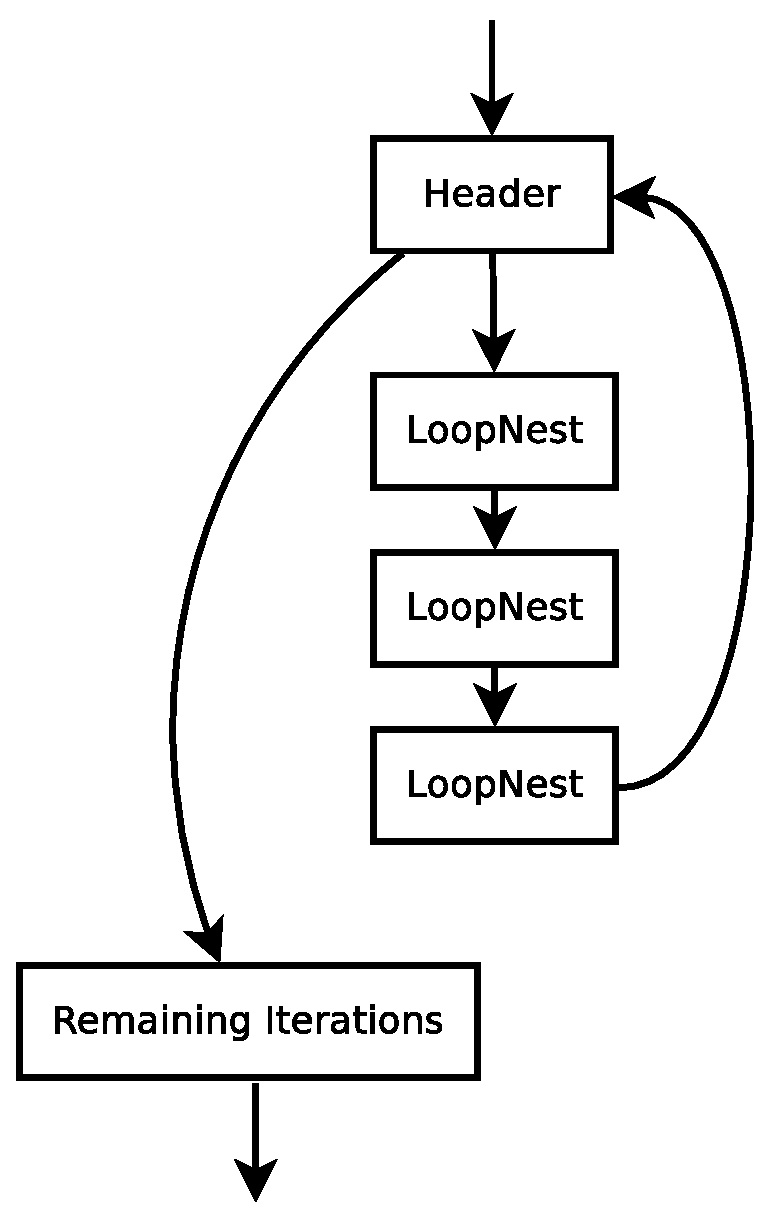
\includegraphics[width=0.7\textwidth]{Figures/ForkJoinCFG.eps}
    \label{fig:ForkJoinCFG} 
    \end{minipage}
  }
  \subfloat[SPolly ParCFG]{
    \begin{minipage}[c][8cm]{0.50\textwidth}
    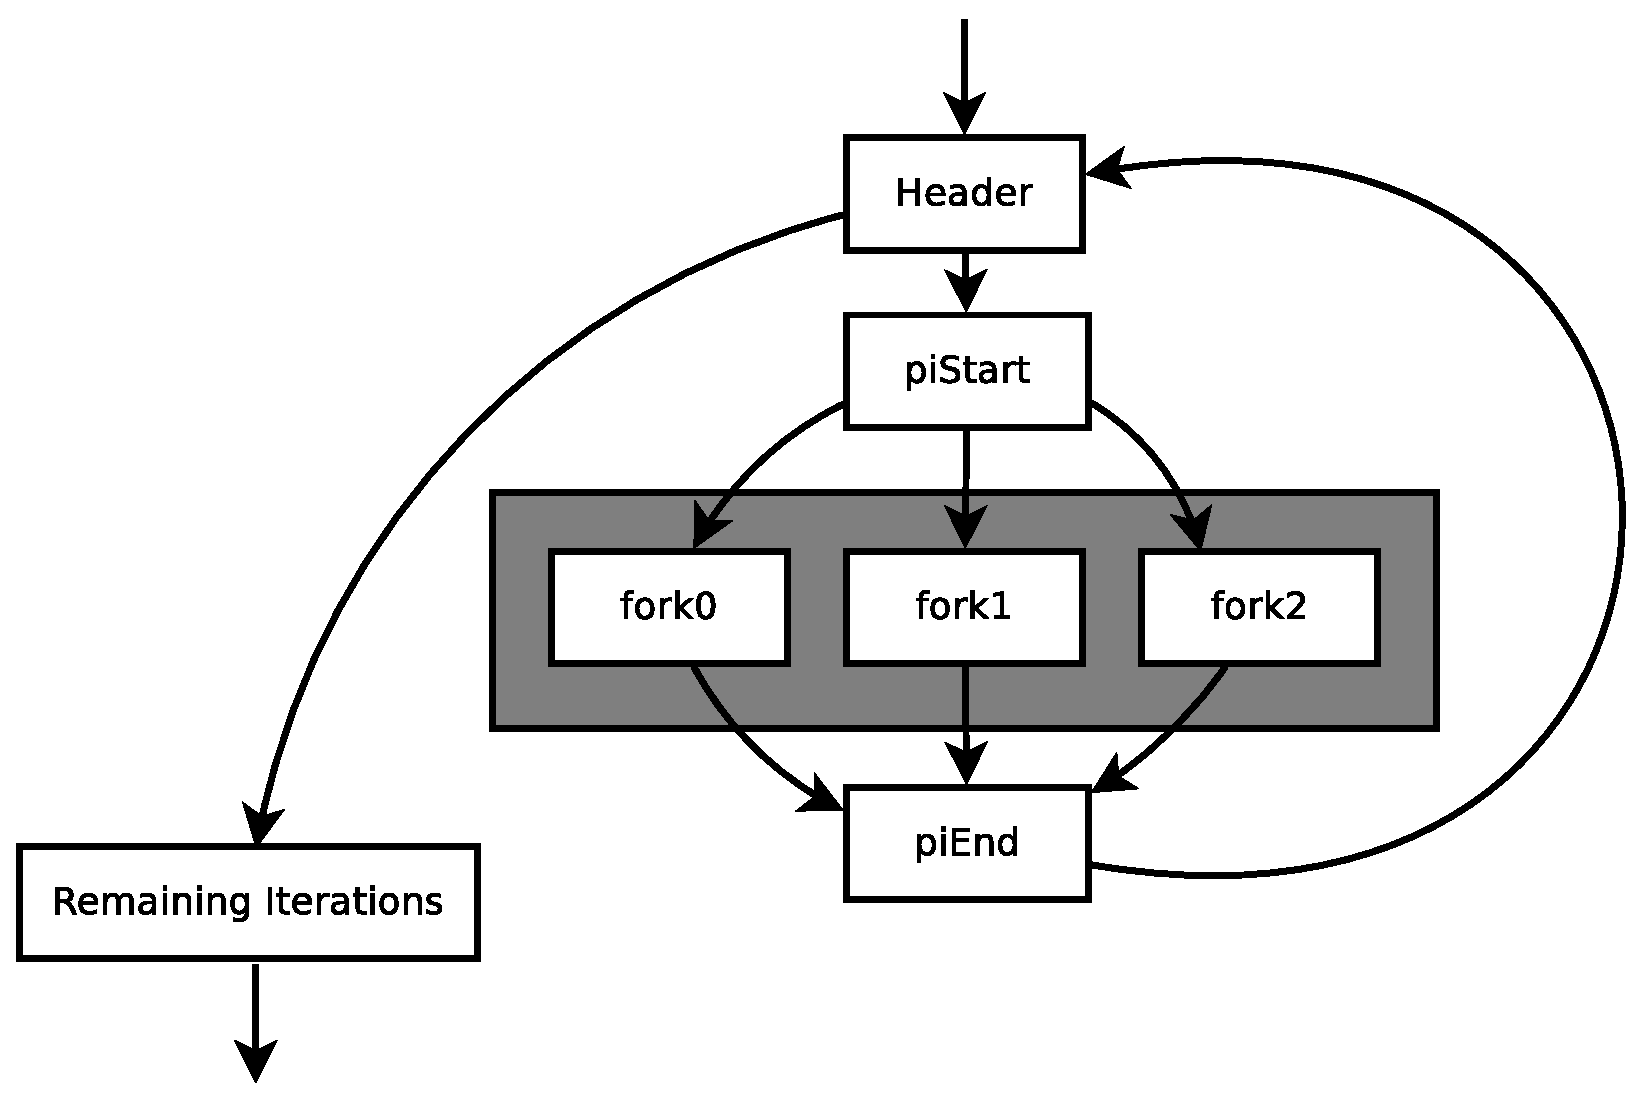
\includegraphics[width=\textwidth]{Figures/ForkJoinParCFG.eps}
    \label{fig:ForkJoinParCFG}
    \end{minipage}
  }
  \caption{Forked CFG produced by SPolly and resulting ParCFG}
  \label{fig:CreateParCFG}  
\end{figure}
\resetlst

\section{Sambama Compile Time Module}
The compile time part of the Sambamba module locates all sSCoPs
within the given input module and transfers each one afterwards in a separated 
function. These extracted sSCoPs are stored within the created Sambamba 
bitcode or respectively executable file. Extracting every single sSCoP 
decreases the performance but allows to easily change and combine different 
optimized sSCoPs, even if they originated from the same function.   
At the moment there is one exception implemented which will be applied on sSCoPs
with complete checks, thus valid SCoPs after the tests are passed. All of those
are optimized in place without consulting the region scores or any other heuristic.
The functionality of the compile time part is minimal but it helps to focus 
on profiling and execution during runtime, without analysis overhead. 
Further work could heavily improve this part, beginning by compile time 
preparation of the sSCoPs, but imaginable is more than just a precomputed
profiling or optimized version of a sSCoP.
As there are a lot of parameters which could have significant impact 
on the performance, several optimized versions of an sSCoP could be created
and stored, in order to choose the best depending on the system and the actual
run, thus depending on runtime information.
While table \ref{tab:PollyOptions} gives a brief
overview of available options for Polly, it is not clear which ones will
fit best for a particular environment and sSCoP. 
As the method versioning system of Sambamba evolves, the compile time part 
should, in order to reduce the workload at runtime and increase the ability to
adapt. 

\section{Sambama Runtime Module}

In addition to the compile time parts, which only rely on static analyses,
the runtime part uses different kinds of runtime information to decide. 
To take advantage of this extra knowledge, most of the decisions, thus most of
the program logic, is implemented in the runtime module. 


Table \ref{}[TODO] gives an overview of the functionalities.


\begin{table}[htbp]
  \caption{Functionality of the SPolly Sambamba module}
  \begin{tabular}{| l |}
    \hline
    
    \hline
    \hline

    \hline
  \end{tabular}
\end{table}



\subsection{Profiling}


\section{Profiling For Sambamba}

Sambamba, as heavily developed research project, was not capable of any kind
of profiling when I started my work. By now, there are two profilers available.
The first one, implemented by the authors of Sambamba, 
is used for exact time measuring, while I created the second one to profiles
executions and data.
[TODO if first is used later on, write it here] Both were
developed during the same time to fulfill different needs and could be
[TODO will be ?]  merged anytime soon. 
As most of SPollys parts are unrelated, to both of them, 
the profiling versions, as their name indicates, would become useless without.
This will definitely increase the number of unnecessary created (parallel) 
functions, but it would not render SPolly redundant.
There a sSCoPs which a guarded by sound checks, thus they can be used with the
overhead of only the check. As the use of other sSCoPs could increase the 
performance too, a heuristic could look for promising candidates, even without
any runtime information. This heuristic could be part of future work since even
with a profiler by hand, there are cases where the gathered information
(see [TODO]) are not helpful at all.



\section{Region Scores}
Initial efforts to create these scores did not use any kind of 
memory, thus the whole region was analysed every time new information was available.
To avoid this unnecessary computations the current score is a
symbolic value which may contain variables for values not known statically, e.g.,
branch probabilities or loop bounds.
Evaluation of these symbolic values will take all profiling 
information into account and yield a comparable integer value. 
Only during the initial score creation the region will be traversed to find
parameters and branches for later annotation. 

All instructions will be scored and the violating ones
will be checked for their speculative potential.
As memory instructions are 
guarded by the STM for the case the speculation failed, calls may not be
reversible, thus without any speculative potential at all. Such function calls
are not checked earlier since the region speculation needs the information about
possible other branches within this region. 
Listing \ref{lst:sSCoPprintf} 
provides such an example but these cases will be revisited in the next 
two chapters too. Table \ref{tab:Scores} lists the scores for the examples in 
figure \ref{fig:ScoredSCoPs}.

 % Evaluation 

% Chapter 5

\chapter{Evaluation} % Write in your own chapter title
\label{Chapter5}
\lhead{Chapter 5. \emph{Evaluation}} % Write in your own chapter title to set the page header

\begin{wraptable}[]{r}{0.36\textwidth}
  \vspace*{-6mm}
  \begin{framed}
  \caption{The evaluation environment}
    \begin{tabular}{ r | c }
      & Machine \\
      \hline
            CPU &  X5570 \\ 
    clock speed & 2.93GHz \\
    L2 cache &  8MB \\
        \#cores &  8 \\
      \#threads &  16 \\
            RAM &  24 GB \\
           LLVM &  3.0 \\
            OS &  Gentoo R7 \\
    \end{tabular}
  \label{tab:EvaluationEnvironment}
  \end{framed}
  \vspace*{-9mm}
\end{wraptable}
SPolly is based on Sambamba and Polly, both research tools under heavy development.
It is hardly surprising that during the implementation of SPolly, 
but also during the evaluation,  problems occurred. 
Even if some of them could be fixed without incurring too much delay, there are still
open problems. On the one hand there are reported bugs (see Table \ref{tab:Bugreports})
which will be resolved in future releases. And on the other hand there is the
current STM implementation in the Sambamba framework which does neither provide
a commit order nor a wait construct, as most general STM implementations do not.
Because of those problems it is currently not possible to handle arbitrary general 
purpose code. Even non-speculative parallelization for SPEC benchmarks will 
certainly cause Polly to crash or to produce invalide code.
Nevertheless, we provide quantitative results on the applicability of 
SPolly on SPEC 2000 benchmarks as well as 
%performance data for the matrix multiplication
%example (in the next Chapter).
%As mentioned, the current state of Polly and Sambamba did not allow us to evaluate SPolly 
%in a proper way, so we provide 
a discussion on the shape and characteristics 
of the detected sSCoPs. For performance data we refere to the next Chapter as it 
contains a detailed evaluation for several versions of the  matrix multiplication example. 

%all detected sSCoPs, we only provide a discussion on (some of the) sSCoPs with complete
%checks detected in the 300.twolf benchmark. 
%In this context ``some'' means exactly three, as for all others Polly will create 
%invalid code according to the reported bugs.  
%We looked only at sSCoPs with complete checks as we can guarantee a sound result 
%with no need of an (extended) STM implementation. 

%As the STM implementation 
%is no problem, Polly is. 
%Furthermore, a detailed case study and evaluation on several versions of the matrix 
%multiplication example is given in the next Chapter.

Information about the environment used for the evaluation but also for the case study 
is given in Table \ref{tab:EvaluationEnvironment}.

%As this  includes the SPEC 2000 benchmark suite, 
%we will shift the evaluation such that most of the runtime evaluation 
%is done for a simpler example. The chosen matrix multiplication has a major benefit. 
%Its popularity allows us to compare the results with related. Due to the 


%\begin{wraptable}[]{r}{0.42\textwidth}
  %\caption{The evaluation environment}
  %\begin{center}
    %\begin{tabular}{ r | c c }
      %& A & B \\
      %\hline
            %CPU & i5 M560 & X5570 \\ 
    %clock speed & 2.67GHz & 2.93GHz \\
    %smart cache & 3MB & 8MB \\
        %\#cores & 2 & 8 \\
      %\#threads & 4 & 16 \\
            %RAM & 6GB & 24 GB \\
           %LLVM & 3.0 debug & 3.0 \\
             %OS & Arch  & Gentoo R7 \\
    %\end{tabular}
  %\end{center}
  %\label{tab:EvaluationEnvironment}
%\end{wraptable}


\section{Quantitative Results}
%The presented quantitative results can be divided into several parts.
%First of all, Polly and SPolly are compared or, to be more precise, 
%the number of detected SCoPs and sSCoPs.
%These results correspond to the applicability of SPolly, 
%as they outline how many additional regions can be speculatively 
%optimized and at least partially parallelized now. 
%Even if the number of speculative SCoPs does not correspond to the amount 
%of exploitable parallelism, future work on Polly, especially 
%the dependency analysis, could allow more SCoPs and sSCoPs (e.g., case E of 
%the case study) to be parallelized.
%Afterwards, the ``quantity'' of the detected sSCoPs is described. Even if we cannot 
%provide a full performance evaluation, this should give hints on the expected 
%results. 

%\subsection{Polly Versus SPolly}

Speculative SCoPs are an extension to ordinary SCoPs, thus we may compare them 
in terms of quantity and the amount of parallelism we can exploit. 
Absolute numbers together with general  
information about the benchmarks are listed in Table 
\ref{tab:TAB}, while a graphical representation is given by Figure \ref{fig:ParallelizableSCoPs}. 
First note that the \textbf{SCoPs} (\textbf{sSCoPs}) column in Table \ref{tab:TAB} contains the 
number of detected SCoPs (sSCoPs) as well as the number of \textit{parallelizable} SCoPs 
(sSCoPs). The other columns provide the number of instructions 
(\textbf{\#instr}), functions (\textbf{\#func}) and simple regions (\textbf{\#sr})
for a particular benchmark.  \\

%The average running time of SPolly is of special interest,
%because the current implementation always computes the initial region score and 
%all  possible tests when an sSCoP is created. A plain comparison with the SCoP detection of 
%Polly. With the exception of the twolf benchmark, SPolly seams to be 
%proportional in the number, but also in the size of the detected scops.
%The number of detected sSCoP has been more than doubled in comparison to Polly,
%a good ratio for the first try to weaken the requirements on SCoPs.

\begin{table}[htbp]
  \centering
  \begin{framed}
  \caption{Results of running Polly and SPolly on SPEC 2000 benchmarks}
  \begin{tabularx}{0.81\textwidth}{l | r | r | r | X | X }
    %\hline
    %\multirow{2}{*}{\textbf{Benchmark}} & \multirow{2}{*}{\textbf{\#func}} & \multicolumn{2}{c|}{\textbf{\#simple regions}} & \multirow{2}{*}{\textbf{\#instr}} &  \multicolumn{2}{c|}{\textbf{valid SCoPs}} &  \multicolumn{2}{c|}{\textbf{Avg detection time}} \\
    \textbf{Benchmark} &\textbf{\#instr} & \textbf{\#func} &\textbf{\#sr} &\centering \textbf{SCoPs}& \textbf{\ sSCoPs} \\
    %\cline{6-9} \cline{3-4}
    %\cline{3-6} 
    \hline
    \hline
  188.ammp   & 19824 & 161 &  208 & 16 \hfill \textit{12}  & 73 \hfill \textit{34}  \\
  179.art    &  1667 &  22 &   66 & 5 \hfill \textit{0}    & 17 \hfill \textit{5}   \\
  256.bzip2  &  3585 &  59 &  116 & 31 \hfill \textit{22}  & 76 \hfill \textit{46}  \\
  186.crafty & 25541 & 105 &  310 & 42 \hfill \textit{30}  & 67 \hfill \textit{52}  \\
  183.equake &  2585 &  24 &   71 & 10 \hfill \textit{9}   & 40 \hfill \textit{36}  \\
  164.gzip   &  4773 &  59 &   95 & 9 \hfill \textit{5}    & 10 \hfill \textit{6}   \\
  181.mcf    &  1663 &  24 &   33 & 2 \hfill \textit{2}    & 2  \hfill \textit{2}   \\
  177.mesa   & 80952 & 769 &  832 & 107 \hfill \textit{79} & 276 \hfill \textit{208}\\
  300.twolf  & 35796 & 166 &  716 & 8 \hfill \textit{4}    & 39 \hfill \textit{20}  \\
  175.vpr    & 19547 & 294 &  329 & 17 \hfill \textit{8}   & 56 \hfill \textit{31}  \\
    %\hline
  \end{tabularx}
  \label{tab:TAB}
  \end{framed}
\end{table}

Regarding only the amount of detected SCoPs and sSCoPs respectively, SPolly is 
able to handle 1.5 times more regions than Polly. Even if this does not
correspond to amount of exploitable parallelism in general, 
it indicates that the applicability of SPolly is very much bigger on general
purpose code. For the particular benchmarks, the number of parallelizable sSCoPs 
is actually 1.5 times greater than the number of parallelizable SCoPs, too.
In this context a SCoP (or sSCoP) is considered as parallelizable if it contains
a loop without loop carried dependencies (modulo the applied speculations; Section \ref{SpeculativeParallelExecution}).

\section{Detected sSCoPs} 
The ``quality'' of  the detected sSCoPs is unfortunately not as desired;  
except three of them, all contain only a single loop and in the majority 
less than 30 LLVM-IR instructions. Even if this is 
comparable to the size of the matrix multiplication example,
the loop trip counts are much smaller. Due to these facts, parallelization causes
more overhead than speedup for most of them. Unsound 
tests (without an STM) substantiate this statement as the performance worsens 
when each sSCoP is speculatively parallelized. 
Even though parallelizing all sSCoPs has negative effects on the overall 
performance, 
the highest ranked sSCoPs are promising candidates for speculation after all. 
Examples for such high ranked candidates are given in Figure \ref{fig:ExampleCandidates}. 
Parts {\footnotesize A}  and {\footnotesize B} present loops with statically 
unknown trip counts, while parts {\footnotesize C} 
and {\footnotesize D} have a statically known iteration counts (64 and 1024, respectively).
All four loops contain possibly aliasing pointers, but only the last one also 
function calls. Note that the function calls in this sSCoP are not guarded by a conditional, 
thus SPolly would currently discard this sSCoP during the initial validation.  
As future work could include (basic) analysis on the called functions, 
the \texttt{exp} function called here could be classified as non-violating,
hence there would be no need to discard this sSCoP. With or without such an analysis, it is 
worth to emphasize that SPolly detects the presented loops automatically 
and ranks them far beyond the average. 


%Even though, we tried to find sSCoPs which can be parallelized 
%(despite the mentioned problems) and yet yield better performance. 
%The picked functions and the results are described in Section \ref{RuntimeResults}. 

\begin{figure}[htbp]
  \centering
  \includegraphics[width=\textwidth]{Figures/parallelizableSCoPs.pdf}
  \caption{Quantity of detected and parallelizable SCoPs and sSCoPs}
  \label{fig:ParallelizableSCoPs}
\end{figure}




\section{Sound Transformations}
\label{soundCTtransformations}
\begin{wraptable}[]{l}{0.4\textwidth}
  \vspace*{-9mm}
  \begin{framed}
  \caption{Number of \\sSCoPs with complete checks}
  \centering
    \begin{tabular}{ l | r }
    \textbf{Benchmark} &  \\
      \hline \hline
  188.ammp   & 6 \\
  183.equake & 5  \\
  177.mesa   & 109  \\
  300.twolf  & 26  \\
  175.vpr    & 3  \\
    \end{tabular}
  \vspace*{-1mm}
  \label{tab:soundTransformations}
  \end{framed}
  \vspace*{-13mm}
\end{wraptable}
For sSCoPs with complete checks, as described earlier, 
there is no need for a runtime system, especially an STM, in order 
to allow sound optimization and parallelization. 
Within the SPEC 2000 benchmarks, SPolly detected 149 sSCoPs with complete checks 
(see Table \ref{tab:soundTransformations}), but attempts to compute performance 
data failed. In the case of e.g., 300.twolf, Polly created valid parallelized code for
3 of the 26 sSCoPs, hence the result is not very representative. As cases B and C
of the matrix multiplication example are sSCoPs with complete checks it is worth 
to look at the case study results when the ``-replace-sound'' option is used. 
A discussion of these results is given in the third paragraph of 
Section \ref{CaseStudyResults}. Also note here that the best result was achieved 
that way.
\\

\lstset{frame=none}
\begin{figure}[htbp]
  \centering
  \vspace*{5mm}
  \subfloat[{ Benchmark: 177.mesa  Function: copy\_tex\_sub\_image}]{
    \begin{minipage}[c]{0.9\textwidth}
    \begin{tabular}{c}
      \lstinputlisting{Primitives/Code/ctsi.c}
    \end{tabular}
  \end{minipage}
  }  
  \vspace*{5mm}

  \subfloat[{Benchmark: 177.mesa  Function: apply\_texture }]{
    \begin{minipage}[c]{0.9\textwidth}
    \begin{tabular}{c}
      \lstinputlisting{Primitives/Code/at.c}
    \end{tabular}
    \end{minipage}
  }
  \vspace*{5mm}

  \subfloat[{Benchmark: 186.crafty Function: InitializeMasks}]{
    \begin{minipage}[c]{0.9\textwidth}
    \begin{tabular}{c}
      \lstinputlisting{Primitives/Code/ia.c}
    \end{tabular}
  \end{minipage}
  } 
  \vspace*{5mm}

  \subfloat[{Benchmark: 300.twolf Function: utemp }]{
    \begin{minipage}[c]{0.9\textwidth}
    \begin{tabular}{c}
      \lstinputlisting{Primitives/Code/utemp.c}
    \end{tabular}
  \end{minipage}
  } 

  \vspace*{5mm}
  \caption{Selection of the highest ranked sSCoPs within the SPEC benchmarks}
  \label{fig:ExampleCandidates}
\end{figure}
\resetlst
%Despite this fact, the approach may yield improvements similar to
%Polly, e.g., for cases B and C of the matrix multiplication case study. 
%Furthermore, a better dependency analysis could allow more parallelism for the 
%detected sSCoPs, as it would allow parallelization of case E in Section \ref{CaseStudyCaseE}.

\clearpage

%\section{Problems}
%During the work with LLVM 3.0 and a corresponding version of Polly a few
%problems occurred. Some of them could not be reproduced in newer versions
%they were just be tackled with tentative fixes, as they will be resolved as soon
%as Sambamba and SPolly will be ported to a newer version.
%Others, which could be reproduced in the current trunk versions,
%have been reported and listed in figure \ref{tab:bugreports}. All bugs were 
%reported with a minimal test case and a detailed description why they occur.
%\clearpage
\section{Backend Evaluation}
\label{Rollbacks}
In the last Chapter we described the two new backends added
to Pollys code generation and we mentioned that both have theirs eligibility.
To substantiate this statement we compared the number of rollbacks for different
loop trip and thread counts when dependencies between iterations occur.
For trip counts of 64 and 1024 we assumed 2 and 16 executing threads respectively.
The dependencies were generated and distributed randomly
with a probability from 0 to 100 percent and last over 1,2 or 16 iterations.
Figures \ref{fig:f64} and \ref{fig:f1024} provide the curves for the geometric mean 
of 1000 iterations without the best and worst 10\%.
The insight gained is the relation between workload per transaction 
(in terms of iterations) and possible amount of needed recomputations. 
The solid line denotes always the blocking backend where each transaction
computes one iteration at a time and the dashed lines denote the splitting backend 
where a transaction computes $\frac{\#iterations}{\#threads}$ iterations. 
In the former case, only one iteration has to be recomputed once a dependency occurs, 
but in the latter case it would be $\frac{\#iterations}{\#threads}$.  Regarding parts 
{\footnotesize A} and {\footnotesize C} of the Figures 
\ref{fig:f64} and \ref{fig:f1024}, we can see that dependencies over only one 
iteration do affect both versions nearly the same. This is hardly 
surprising as the probability to recompute a transaction in the splitted version
is decreased by the factor $\frac{\#iterations}{\#threads}$ and once it is rolled
back exactly the same number of iterations have to be recomputed. For such cases,
the preferred version would be the splitted one, because the additional overhead
due to e.g., synchronization, is far less 
(again by a factor of $\frac{\#iterations}{\#threads}$). 
The situation changes as the dependencies last over more iterations, as indicated
by the parts {\footnotesize B} and {\footnotesize D}. The overhead for the
blocked and unrolled version stays the same but the splitted version suffers from
more rollbacks as now each dependency forces a transaction to recompute. The 
factor decreasing the probability was $\frac{\#iterations}{\#threads}$,
hence the curves in the Figures \ref{fig:ff6422} and \ref{fig:ff102422} 
are, at the beginning, shifted up by 2 and the ones in Figures \ref{fig:ff641616}
and \ref{fig:ff10241616} by 16. As the asymptotic behaviour of both versions 
is the same, the graphs will always converge with increasing dependency probability.
In the presented examples, this behaviour only matters after the probability for dependencies
reached about 90\%. Beyond this limit, the distance between the two graphs is rapidly 
decreasing. 

Summarized, both versions have advantages and drawbacks which needed to be considered
for speculative execution. A blocked and unrolled version might not provide
the desired speedup but nevertheless hints on the probability of occurring dependencies
and even their ``size''. Such information could suggest a second parallelized 
version e.g., with more workload per transaction, if it would exceed the first
one in terms of speedup but with a acceptable probability of overhead.
%if the expected speedup would exceed the probability 

\begin{figure}[htbp]
      \vspace*{-5mm}
  \centering
  \subfloat[64 iterations, 2 threads, dependencies over 1 iteration]{
    \begin{minipage}[c]{0.43\textwidth}
      \includegraphics[width=\textwidth]{Figures/missesUnique6421.eps}
      \label{fig:ff6421}
      \vspace*{-5mm}
    \end{minipage}
  }
  \subfloat[64 iterations, 2 threads, dependencies over 2 iteration]{
    \begin{minipage}[c]{0.43\textwidth}
      \includegraphics[width=\textwidth]{Figures/missesUnique6422.eps} 
      \vspace*{-5mm}
      \label{fig:ff6422}
    \end{minipage}
  }

      \vspace*{-5mm}
  \subfloat[64 iterations, 16 threads, dependencies over 1 iteration]{
    \begin{minipage}[c]{0.43\textwidth}
      \includegraphics[width=\textwidth]{Figures/missesUnique64161.eps}
      \label{fig:ff64161}
      \vspace*{-5mm}
    \end{minipage}
  }
  \subfloat[64 iterations, 16 threads, dependencies over 16 iteration]{
    \begin{minipage}[c]{0.43\textwidth}
      \includegraphics[width=\textwidth]{Figures/missesUnique641616.eps}
      \label{fig:ff641616}
      \vspace*{-5mm}
    \end{minipage}
  }
  \caption{Backend evaluation with 64 iterations}
  \label{fig:f64}
\end{figure}

%\begin{figure}[htbp]
  %\centering
  %\subfloat[128 iterations and 2 threads]{
    %\begin{minipage}[c]{0.45\textwidth}
      %\includegraphics[width=\textwidth]{Figures/misses1282.eps}
      %\label{lst:ff1282}
    %\end{minipage}
  %}
  %\subfloat[128 iterations and 4 threads]{
    %\begin{minipage}[c]{0.45\textwidth}
      %\includegraphics[width=\textwidth]{Figures/misses1284.eps} 
      %\label{lst:ff1284}
    %\end{minipage}
  %}

  %\subfloat[128 iterations and 8 threads]{
    %\begin{minipage}[c]{0.45\textwidth}
      %\includegraphics[width=\textwidth]{Figures/misses1288.eps}
      %\label{lst:ff1288}
    %\end{minipage}
  %}
  %\subfloat[128 iterations and 16 threads]{
    %\begin{minipage}[c]{0.45\textwidth}
      %\includegraphics[width=\textwidth]{Figures/misses12816.eps}
      %\label{lst:ff12816}
    %\end{minipage}
  %}
  %\caption{Backend evaluation with 128 iterations}
  %\label{fig:f128}
%\end{figure}


%\begin{figure}[htbp]
  %\centering
  %\subfloat[256 iterations and 2 threads]{
    %\begin{minipage}[c]{0.45\textwidth}
      %\includegraphics[width=\textwidth]{Figures/misses2562.eps}
      %\label{lst:ff2562}
    %\end{minipage}
  %}
  %\subfloat[256 iterations and 4 threads]{
    %\begin{minipage}[c]{0.45\textwidth}
      %\includegraphics[width=\textwidth]{Figures/misses2564.eps} 
      %\label{lst:ff2564}
    %\end{minipage}
  %}

  %\subfloat[256 iterations and 8 threads]{
    %\begin{minipage}[c]{0.45\textwidth}
      %\includegraphics[width=\textwidth]{Figures/misses2568.eps}
      %\label{lst:ff2568}
    %\end{minipage}
  %}
  %\subfloat[256 iterations and 16 threads]{
    %\begin{minipage}[c]{0.45\textwidth}
      %\includegraphics[width=\textwidth]{Figures/misses25616.eps}
      %\label{lst:ff25616}
    %\end{minipage}
  %}
  %\caption{Backend evaluation with 256 iterations}
  %\label{fig:f256} 
%\end{figure}

%\begin{figure}[htbp]
  %\centering
  %\subfloat[512 iterations and 2 threads]{
    %\begin{minipage}[c]{0.45\textwidth}
      %\includegraphics[width=\textwidth]{Figures/misses5122.eps}
      %\label{lst:ff5122}
    %\end{minipage}
  %}
  %\subfloat[512 iterations and 4 threads]{
    %\begin{minipage}[c]{0.45\textwidth}
      %\includegraphics[width=\textwidth]{Figures/misses5124.eps} 
      %\label{lst:ff5124}
    %\end{minipage}
  %}

  %\subfloat[512 iterations and 8 threads]{
    %\begin{minipage}[c]{0.45\textwidth}
      %\includegraphics[width=\textwidth]{Figures/misses5128.eps}
      %\label{lst:ff5128}
    %\end{minipage}
  %}
  %\subfloat[512 iterations and 16 threads]{
    %\begin{minipage}[c]{0.45\textwidth}
      %\includegraphics[width=\textwidth]{Figures/misses51216.eps}
      %\label{lst:ff51216}
    %\end{minipage}
  %}
  %\caption{Backend evaluation with 512 iterations}
  %\label{fig:f512}
%\end{figure}

\begin{figure}[htbp]
      \vspace*{-5mm}
  \centering
  \subfloat[1024 iterations, 2 threads, dependencies over 1 iteration]{
    \begin{minipage}[c]{0.43\textwidth}
      \includegraphics[width=\textwidth]{Figures/missesUnique102421.eps}
      \label{fig:ff102421}
      \vspace*{-5mm}
    \end{minipage}
  }
  \subfloat[1024 iterations, 2 threads, dependencies over 2 iteration]{
    \begin{minipage}[c]{0.43\textwidth}
      \includegraphics[width=\textwidth]{Figures/missesUnique102422.eps} 
      \label{fig:ff102422}
      \vspace*{-5mm}
    \end{minipage}
  }

      \vspace*{-5mm}
  \subfloat[1024 iterations, 16 threads, dependencies over 1 iteration]{
    \begin{minipage}[c]{0.43\textwidth}
    \includegraphics[width=\textwidth]{Figures/missesUnique1024161.eps}
      \label{fig:ff1024161}
      \vspace*{-5mm}
    \end{minipage}
  }
  \subfloat[1024 iterations, 16 threads, dependencies over 16 iteration]{
    \begin{minipage}[c]{0.43\textwidth}
      \includegraphics[width=\textwidth]{Figures/missesUnique10241616.eps}
      \label{fig:ff10241616}
      \vspace*{-5mm}
    \end{minipage}
  }
  \caption{Backend evaluation with 1024 iterations}
  \label{fig:f1024}
\end{figure}
 % Results and Discussion

% Chapter 6

\chapter{Case Study} % Write in your own chapter title
\label{Chapter6}
\lhead{Chapter 6. \emph{Case Study}} % Write in your own chapter title to set the page header


\section{Matrix Multiplication}
\label{MatrixMultiplication}
Matrix multiplication is a well known computational problem and part of many 
algorithms and programs, e.g., ammp within the SPEC 2000 benchmark suite.
If the data size grows, the runtime may have crucial impact on the
overall performance. Tiling, vectorization and parallel execution yield an
enormous speedup as different approaches already
showed\cite{grosser:thesis, JIMBOREAN-2012-664345},
still the question of applicability remains. A slightly modified source code 
may not be optimized at all, even if the computation has not been changed. 

\paragraph{Measurement} ~\\
This Chapter will compare different implementations of a simple 2d
matrix multiplication for a sample size of  $1024*1024$ floats.
Each example is executed $100$ times and the geometric mean of the results 
(without the best and worst 10\%) is computed. All numbers are generated on 
the machine described in Table \ref{tab:EvaluationEnvironment}. 
If not mentioned explicitly, the base
algorithm remains the same for each case, so there is no hand made optimization 
involved. Furthermore, no hand made optimizations are applied on intermediate 
results, thus the outcome is only dependent on the input and the presented 
options. To prevent false optimizations the result is validated after each iteration.

\paragraph{Notes} ~\\
Even if the STM embedded into the Sambamba framework does
not provide a commit order yet, SPolly will speculatively execute loops in
parallel. For the matrix multiplication example with proper inputs 
this is sound. Furthermore, SPolly is able to create sound versions for the cases 
A to C because the alias tests for these cases are complete. 

%As the last problems during this evaluation have been originated
%in the STM we turned it completely off for the whole case study. 
%This will obviously not reflect the introduced overhead, but it provides the tenor
%as well as for the
%current implementation of the parallelizer. 


\clearpage
\lstset{frame=none}
\subsection*{Case A} 
\label{CaseStudyCaseA}
\begin{wrapfigure}[]{r}{0.5\textwidth}
  \centering
    \hfill
    \hfill
    \begin{minipage}[c]{0.4\textwidth}
    \vspace*{-7mm}
    \lstinputlisting{Primitives/Code/matmul1prep.c}
    \end{minipage}
    \hfill
    \hfill
    \vspace*{-2mm}
    \caption{Matrix multiplication case A}
   \label{lst:MatmulVersionA}
\end{wrapfigure}

Figure \ref{lst:MatmulVersionA} shows the matrix multiplication as used in 
many presentations and benchmarks. This case is quite grateful because the
global arrays are disjoint and fixed in size. Furthermore, the loop nest is
perfectly nested and all memory accesses can be computed statically.
With this in mind the popularity of this case is hardly surprising,
just as the outstanding results are.


\subsection*{Case B} 
\begin{wrapfigure}[]{l}{0.5\textwidth}
    \begin{minipage}[c]{0.4\textwidth}
    \vspace*{-7mm}
    \lstinputlisting{Primitives/Code/matmul2prep.c}
    \end{minipage}
    \hfill
    \hfill
    \vspace*{-2mm}
    \caption{Matrix multiplication case B}
    \label{lst:MatmulVersionB}
    \vspace*{-8mm}
\end{wrapfigure}

Case B (see Figure \ref{lst:MatmulVersionB}) is very similar to the previous one.
The arrays are still fixed in size but now given as arguments. Even if the
declaration is still global, common alias analysis can not prove the independence
of each array anymore. Summarized aliasing between \texttt{A,B} and \texttt{C} 
is possible.  \\

\subsection*{Cases C and D} 
Cases C and D as presented in Figures \ref{lst:MatmulVersionC} and 
\ref{lst:MatmulVersionD} are using pointers instead of fixed size arrays. 
This common practice to generalize the computation suffers from the same 
disadvantages as the second case. Common alias analyses will provide insufficient
information to optimize the loop nest. In the context of this work case D is 
of special interest as it does not allow conclusive alias tests in front of the
loop nest.  

\clearpage
\begin{figure}[htpb]
  \centering
  \subfloat[Matrix multiplication case C] {
    \hfill
    \hfill
    \begin{minipage}[c][6cm]{0.4\textwidth}
    \lstinputlisting{Primitives/Code/matmul3prep.c}
    \end{minipage}
    \hfill
    \hfill
   \label{lst:MatmulVersionC}
  }
  \hfill
  \subfloat[Matrix multiplication case D] {
    \hfill
    \hfill
    \begin{minipage}[c][6cm]{0.4\textwidth}
    \lstinputlisting{Primitives/Code/matmul4prep.c}
    \end{minipage}
    \hfill
    \hfill
    \label{lst:MatmulVersionD}
  }
  \caption{Matrix multiplication case C and D}
   \label{lst:MatmulVersionCD}
\end{figure}


\subsection*{Case E} 
\label{CaseStudyCaseE}
\begin{wrapfigure}[]{r}{0.5\textwidth}
    \hfill
    \hfill
  \begin{minipage}[c]{0.4\textwidth}
    \vspace*{-7mm}
    \lstinputlisting{Primitives/Code/matmul5prep.c}
    \end{minipage}
    \hfill
    \hfill
    \caption[Matrix multiplication case E]{Matrix multiplication case E, extracted from the ammp benchmark (SPEC 2000)}
    \vspace*{-5mm}
    \label{lst:MatmulVersionE}
\end{wrapfigure}
The last case we will look at is the matrix multiplication within the ammp 
benchmark. It is similar to case D but with manual optimizations which could
be performed by clang (and therefore by Polly and SPolly) too, if type based alias
information is available. The particular differences between case D and
E are the lifted index computations and the strength reduction on the innermost
loop.  A stripped version of the original source code is given in 
Figure \ref{lst:MatmulVersionE}.  Even if the algorithm stays the same, 
the accesses functions are substantially altered. Polly 
will not recognize them as affine anymore, hence they will be overestimated. The resulting 
polyhedral representation has loop carried dependencies between all iterations in 
every loop. Polly cannot and SPolly will not parallelize a loop based on these 
information. Future work on SPolly could allow to
distinguish between encountered and overestimated 
dependencies. This would allow more speculation but it remains to determine when this is useful. 

%\clearpage
\subsection{Results and Discussion}
\label{CaseStudyResults}
Regarding the results in Table \ref{tab:CaseStudyResults}, SPolly 
achieve up to 80 fold speedup compared to gcc and clang; Polly, with the
default options, only 34 fold speedup. 
Although smaller input data will not yield improvements in such dimensions, 
the tenor remains. SPolly as presented here is at least as effective as
Polly but with much wider applicability. 
It is able to parallelize the cases A to C in a sound way 
without manual interaction. 
Case D is special, as speculation is needed to parallelize it. Nevertheless, 
the execution with SPolly yields more than 8x speedup (without an STM).
Polly, on the other hand, can only handle case A. With the assumption
that no pointers alias it is able to optimize and parallelize cases B and C, too.
As this is obviously not
true in general, the source has to be reviewed manually to enable such optimizations. 
Apart from the parallization, the cases A to C could benefit from the 
polyhedral transformation, hence from improved data-locality. 
Comparing, for example, the results of case C and D when parallelized with Sambamba, 
this yields an addional 3 fold speedup.

\paragraph*{Parallelized versions} ~\\
Comparing the different parallelized versions of the cases A, B and C in terms of execution time,
the OpenMP version created by SPolly performed  best, but only on large tile sizes. 
The OpenMP versions almost always perform better than the ones parallelized by Sambamba, 
likely because of the transaction queue approach still used for the evaluation of this work.
We expect better results with the TBB\cite{Corporation_2008} implementation as 
described earlier. Nevertheless, Sambamba and its parallelizer are needed to 
handle case D in the first place. And once the commit order is 
implemented, the STM will be used to secure the execution for arbitrary input.

\paragraph*{SPollys sSCoP replacement} ~\\
As SPolly utilizes only Polly functionalities (without any speculation)
when the ``-replace-sound'' option is used, it is at first surprising that the 
results for those cases differ compared to Pollys. To explain this we have to 
look at the given options in more detail. Polly is designed to be used with O3 as 
done here, but SPolly is not. It only utilizes the scheduling and code
generation pass of Polly for optimizations. 
When they are invoked by hand (without O3), 
Polly yields the same results for case A, in fact the execution time will not
differ. We may conclude that for this case 
the introduced alias tests do not cause measurable overhead. 
\\

\paragraph*{Backend comparison} ~\\
Except for a tile size of 256, there is almost no difference between the 
execution times for both new code generation backends, but for this special 
tile size only the splitting backend is currently able to exploit parallelism. 
When the trip count of the first parallelizable loop is less than used 
thread count, here 16,  the blocked and unrolled loop nest version
will not be executed at all, instead the computation is done by the ``remaining iterations loop'' as indicated in Figure \ref{fig:CreateParCFG}. The reason is the single bounds check right 
before the 16 forks/iterations which form the parallel section.
Using the splitting backend, the first 4 of the 16 created loop nests 
will be executed concurrently while the others are skipped. 
Despite the fact that only one fourth of the possible parallelism was exploited, 
we achieved a good result for this particular case. Even the version created by 
the blocking backend was twice as fast as the gcc and clang versions. The reason
is the improved data-locality for the two inner loops.


\paragraph*{Summary} ~\\
Even for this small case study it is hard to talk about ``the'' best parallelization method.
Regarding only the tile size we can see an enormous impact on the runtime for 
some of the cases (Polly case A or SPolly with ``replace sound'') but it is still
unclear whether other, not yet tested values may yield better results. 
In the general case many options and combinations could perform surprisingly well. 
For long running programs it might be imaginable that SPolly internally 
creates a table similar to the presented one. 
Promising options and combinations to create fast versions could be tried 
as well as specialized versions which are only intended for certain inputs.  

%As described earlier, it would be possible to place several well performing versions
%side by side in one CFG. The split block, currently used only for the introduced
%tests, could additionally dispatch each input to  the most suitable version. 

%\paragraph*{Open Work -- Case E} ~\\
%The matrix multiplication extracted from ammp could not be optimized by Polly nor 
%by SPolly because of the hand made optimizations. Even if SPolly detects a sSCoP
%here, parallelization is not possible since Polly overestimates the memory accesses 
%within the loop. Further work on the dependency detection would allow SPolly to 
%extract parallelism for this case too. \\

%less surprising is that polly, while ignoring
%aliases, produces the same results as spolly with 
%the ``sound replacement'' versions. as the produced code is, except a small 
%alias check in front of the loop nest, identical, other results would have been
%strange. 

\clearpage

~\\
\vfill
\vfill
\vfill
\vfill
%\begin{table}[htpb]
  %\begin{framed}
    %\centering
    %\caption[Execution times for the different matrix multiplication cases]{Execution times for the different matrix multiplication examples. 
  %All data is provided in milliseconds for an input size of $1024 * 1024$ floats.}
  %\label{tab:CaseStudyResults}
  %\begin{tabular}{ c |  c | c | c | c | c | l | r}
    %Optimizer & A & B & C &  D & E & Options & tile size\\
    %\hline
    %\hline
    %gcc     & 9221 & 9130  & 9154 &  8917 & 8926 &  best of O1, O2, O3   \\ 
    %clang   & 9268 & 9289  & 9180 &  9315 & 8376 &  best of O1, O2, O3   \\ 
    %Polly   & 240 & "     & "    &  "  & " & 
    %O3, polly\footnotemark[1] (tile-size=8) \\  
    %Polly   & 264 & "     & "    &  " &  "  &  
    %O3, polly\,\,\, (tile-size=16)  \\  
    %Polly   & 269 & "     & "    &  " &  "  &
    %O3, polly\,\,\, (tile-size=32)  \\  
    %Polly   & 348 & "     & "    &  " &  "  &
    %O3, polly\,\,\, (tile-size=64)  \\  
    %Polly   & 926 & "     & "    &  " &  "  &
    %O3, polly\,\,\, (tile-size=256)  \\  
    %%Polly   &  "   &  1080 & 1077 &   Err\footnotemark[5]   &  "   &  OpenMP, ia\footnotemark[2]  \\  
    %%Polly   &  114 &  115  & 115  &   Err &  "  &  isl, ts 256, OpenMP, ia   \\  
    %%Polly   &  331 &  328  & 334  &   Err &  "  &  isl, ts 32,  OpenMP, ia  \\  
    %SPolly  &  & 377 & 365  &  "  &  "  &  isl\footnotemark[2], OpenMP, rs\footnotemark[3], (tile-size=8)  \\  
    %SPolly  &  & 370 & 349  &  "  &  "  &  isl,\,\: OpenMP, rs,\,\; (tile-size=16)   \\  
    %SPolly  &  & 382 & 354  &  "  &  "  &  isl,\,\: OpenMP, rs,\,\; (tile-size=32)   \\  
    %SPolly  &  & 520 & 473  &  "  &  "  &  isl,\,\: OpenMP, rs,\,\; (tile-size=64)   \\  
    %SPolly  &  & 114 & 114  &  "  &  "  &  isl,\,\: OpenMP, rs,\,\; (tile-size=256)   \\  
    %SPolly  & 364 & 369 & 351  & 1110 & "& spolly, sp,\,\, bb\footnotemark[4], (tile-size=8) \\  
    %SPolly  & 371 & 365 & 342  & " &"& spolly, sp,\,\, bb,\,\; (tile-size=16) \\  
    %SPolly  & 377 & 373  & 345 & " &"& spolly, sp,\,\, bb,\,\; (tile-size=32) \\  
    %SPolly  & 514 & 510  & 458  & " &"& spolly, sp,\,\, bb,\,\;  (tile-size=64) \\  
    %SPolly  & 4636 & 4630 & 4179 & " &"& spolly, sp,\,\, bb,\,\; (tile-size=256) \\  
    %SPolly  & 363 & 363 & 350 & 1111 &  "  & spolly, sp\footnotemark[5], sb\footnotemark[6], (tile-size=8) \\  
    %SPolly  & 359 & 362 & 344 & " &  "  & spolly, sp,\,\, sb,\:\; (tile-size=16) \\  
    %SPolly  & 371 & 371 & 355 & " &  "  & spolly, sp,\,\, sb,\:\; (tile-size=32) \\  
    %SPolly  & 509 & 503 & 460 & " &  "  & spolly, sp,\,\, sb,\:\;  (tile-size=64) \\  
    %SPolly  & 584 & 541 & 456 & " &  "  & spolly, sp,\,\, sb,\:\; (tile-size=256) \\  
    %%SPolly  &  405 &  406  & 418  &     &    & isl, tile size 64, speculative parallelization \\ 
  %\end{tabular}
   
  %\end{framed}
%\end{table}

\begin{table}[h]
  \begin{framed}
    \centering
    \caption[Execution times for the different matrix multiplication cases]{Execution times for the different matrix multiplication examples. 
  All data is provided in milliseconds for an input size of $1024 * 1024$ floats.}
  \label{tab:CaseStudyResults}
  \begin{tabular}{ c |  c | c | c | c | c | c | c}
    Optimizer & A & B & C &  D & E & Options & Tile Size\\
    \hline
    \hline
    gcc     & 9221 & 9130  & 9154 &  8917 & 8926 &  best of O1, O2, O3 &  \\ 
    clang   & 9268 & 9289  & 9180 &  9315 & 8376 &  best of O1, O2, O3& \\ 
    \hline
    Polly   & 240 & 9289  & 9180 & 9315 & 8376 & 
    O3, polly\footnotemark[1] & 8\\  
    Polly  & 264 & 9289 & 9180 & 9315 &  8376 &  
    O3, polly\;\, & 16\\  
    Polly   & 269 & 9289 & 9180 & 9315 &  8376 &
    O3, polly\;\, & 32\\  
    Polly   & 348 & 9289 & 9180 & 9315 & 8376  &
    O3, polly\;\, & 64\\  
    Polly   & 926 & 9289 &  9180& 9315 & 8376  &
    O3, polly\;\, & 256 \\  
    %Polly   &  "   &  1080 & 1077 &   Err\footnotemark[5]   &  "   &  OpenMP, ia\footnotemark[2]  \\  
    %Polly   &  114 &  115  & 115  &   Err &  "  &  isl, ts 256, OpenMP, ia   \\  
    %Polly   &  331 &  328  & 334  &   Err &  "  &  isl, ts 32,  OpenMP, ia  \\  
    SPolly  & 377 & 377 & 365  & 9180 & 8376 & isl\footnotemark[2], OpenMP, rs\footnotemark[3] & 8\\  
    SPolly  & 371 & 370 & 349  & 9180 & 8376 & isl,\,\: OpenMP, rs\;\,  & 16\\  
    SPolly  & 378 & 382 & 354  & 9180 & 8376 & isl,\,\: OpenMP, rs\;\, & 32\\  
    SPolly  & 517 & 520 & 473  & 9180 & 8376 & isl,\,\: OpenMP, rs\;\,   & 64\\  
    SPolly  & 1044 & 114 & 114 & 9180 & 8376 & isl,\,\: OpenMP, rs\;\,  & 256\\  
    SPolly  & 364 & 369 & 351  & 1110 & 8376 & spolly, sp\footnotemark[4], bb\footnotemark[5] & 8\\  
    SPolly  & 371 & 365 & 342  & 1110 & 8376 & spolly, sp,\,\, bb\;\, & 16\\  
    SPolly  & 377 & 373  & 345 & 1110 & 8376 & spolly, sp,\,\, bb\;\, &32\\  
    SPolly  & 514 & 510  & 458  & 1110 & 8376 & spolly, sp,\,\, bb\;\,& 64\\  
    SPolly  & 4636 & 4630 & 4179 & 1110 & 8376 & spolly, sp,\,\, bb\;\,& 256\\  
    SPolly  & 363 & 363 & 350 & 1111 & 8376 & spolly, sp,\,\, sb\footnotemark[6]& 8\\  
    SPolly  & 359 & 362 & 344 & 1111 & 8376 & spolly, sp,\,\, sb\;\,& 16\\  
    SPolly  & 371 & 371 & 355 & 1111 & 8376 & spolly, sp,\,\, sb\;\, & 32\\  
    SPolly  & 509 & 503 & 460 & 1111 & 8376 & spolly, sp,\,\, sb\;\,& 64\\  
    SPolly  & 584 & 541 & 456 & 1111 & 8376 & spolly, sp,\,\, sb\;\, & 256\\  
    %SPolly  &  405 &  406  & 418  &     &    & isl, tile size 64, speculative parallelization \\ 
  \end{tabular}
   
  \end{framed}
\end{table}

\vfill
\vfill
\vfill
\rule{\textwidth}{0.1mm}
\footnotemark[1] -polly -enable-polly-openmp -enable-polly-vector (isl\footnotemark[2] included)\\
\footnotemark[2] -polly-opt-isl, enables isl based tiling and scheduling  \\
\footnotemark[3] Replace sSCoPs with parallel OpenMP versions if checks were sound.  For this evaluation no alias analysis was used, instead alias tests are introduced each time.    \\
\footnotemark[4] parallelized with Sambamba  \\
\footnotemark[5]  blocking backend \\
\footnotemark[6]  splitting backend  

%\begin{figure}[htpb]
  %\centering
  %\subfloat[Matmul version 1]{

  %} \hfill
  %\subfloat[Matmul version 2]{
    %\begin{minipage}[c]{0.45\textwidth}
    %\lstinputlisting{Primitives/Code/matmul2prep.c}
    %\label{lst:MatmulVersion2}
    %\end{minipage}
  %}

  %\subfloat[Matmul version 3]{
    %\begin{minipage}[c]{0.45\textwidth}
    %\lstinputlisting{Primitives/Code/matmul3prep.c}
    %\label{lst:MatmulVersion3}
    %\end{minipage}
  %}
  %\hfill
  %\subfloat[Matmul version 4]{
    %\begin{minipage}[c]{0.45\textwidth}
    %\lstinputlisting{Primitives/Code/matmul4prep.c}
    %\label{lst:MatmulVersion4}
    %\end{minipage}
  %}
  %\caption{Matrix multiplication in different versions }
%\end{figure}
 % Case study

% Chapter 7

\chapter{Conclusion and Future Work} % Write in your own chapter title
\label{Chapter7}
\lhead{Chapter 7. \emph{Conclusion and Future Work}} % Write in your own chapter title to set the page header
%As this work was only the first step towards speculative polyhedral optimization
%there is still open work and ideas not implemented yet. Nevertheless, we think 
%that SPolly, as presented here, already provides sufficient evidences for the
%benefits of this approach.

%The approach benefits not only from the underlying polyhedral model but also from
%the concepts presented in chapter \ref{Chapter3}. 
%The widened applicability and the features offered by Sambamba 
%might be reasons to think about more aggressive specializations at this point in time.


\section{Future Work}
The preceding Chapters already mentioned several possible approaches for future work 
but it is worth to summarize and supplement the list. 

The Sambamba framework and especially the method versioning is designed for 
multiple specialized versions of a single function.
Up to this point there is still open work in this context,
both on the side of Sambamba and of SPolly. For the latter one 
preparations have already been made to catch up when the method versioning 
implementation of Sambamba proceeds. 
The sSCoP extraction explained in Section \ref{sSCoPExtraction} allows multiple
loop nest optimizations and specializations with minimal costs in terms of space
as well as for analyses and transformations. Once a SCoP is extracted, the 
new created function is well suited for local transformations.
Parameters,  e.g., for loop trip counts, could be replaced by constants if
profiling information indicated a certain probability for such a case.
Furthermore, SPolly could create multiple optimized versions of the same sSCoP
using  different options and values e.g., for the tile size.
The case study indicated  that changes for just this particular value may have
significant impact on the performance (3.35x faster compared to the default value).
Considering now the vector width or the fusion strategy, it is unclear whether 
changes could yield similar speedups for certain, not yet investigated, situations. 
Apart from specialization, future work could allow SPolly to differentiate between
real and overestimated dependencies or, to be more precise, it could allow SPolly 
to remove the overestimated dependencies during the code generation. This 
approach would certainly exploit more parallelism but still restrict
the level of speculation. Furthermore, all speculative approaches could benefit 
from improved profiling, especially dependency profiling seems plausible in this context. 



%\begin{table}[htpb]
  %\begin{framed}
    %\centering
    %\caption{Possible specializations for sSCoPs}
  %\label{tab:FutureWork1}
  %\begin{tabular}{l | c | }
    
  %\end{tabular}
  %\end{framed}
%\end{table}


\section{Conclusion}
SPolly is a speculative extension for the polyhedral optimizer Polly which 
improves the applicability and provides first specialization approaches. The
key concepts are not fully usable yet, but still effective. 
Compared to Polly, SPolly reveals 1.5x more parallelizable loops 
on the SPEC 2000 benchmarks and it is able to exploit more parallelism,
even in the absence of Sambamba and an STM.
Used as a non-speculative optimizer SPolly utilizes the functionality of 
Polly and combines it with complete alias checks to secure the parallel execution.
As this behaviour is only a spin-off, the real strength of SPolly lies in the speculation. 
Region scores, the heuristic used to rank detected sSCoPs, combine static information
with profiling data and the results of the introduced checks. Based on these ranks,
SPolly will not only create a speculatively parallelized version for promising 
sSCoPs but also utilize the strength of the polyhedral model to improve their 
data-locality. 

In the context of the case study, SPolly shows that both parallelization and 
polyhedral optimization can be effectively combined with speculation to improve 
their applicability and the performance for more realistic versions of the 
matrix multiplication example. Based on these results it is eligible to state 
SPolly as an effective extension to the polyhedral optimizer Polly, but
with wider applicability on general purpose code and even better results for the 
matrix multiplication.
 % Conclusion

%\input{./Chapters/Chapter} % Future work

%% ----------------------------------------------------------------
% Now begin the Appendices, including them as separate files

%% ----------------------------------------------------------------
\clearpage
\lhead{\emph{List of Figures}}  % Set the left side page header to "List if Figures"
\listoffigures  % Write out the List of Figures

%% ----------------------------------------------------------------
\lhead{\emph{List of Tables}}  % Set the left side page header to "List of Tables"
\listoftables  % Write out the List of Tables
\clearpage

%% ----------------------------------------------------------------
%\lhead{\emph{List of Listings}}  % Set the left side page header to "List of Listings"
%\renewcommand*{\lstlistingname}{List of Listings}
%\lstlistoflistings % Write out the List of Listings 
%\clearpage


\addtocontents{toc}{\vspace{2em}} % Add a gap in the Contents, for aesthetics

\appendix % Cue to tell LaTeX that the following 'chapters' are Appendices

% Appendix A

\chapter{Matrix Multiplication Example}
\label{AppendixA}
\lhead{Appendix A. \emph{Matrix Multiplication Example}}
	% Appendix Title

% Appendix A

\chapter{Polly -- Optimization Options}
\label{AppendixB}
\lhead{Appendix B. \emph{Polly -- Optimization Options}}

Different options may yield different results. Since this simple truth holds for
Polly too, the options, listend in the Table below, may yield improvements even
for already well performing SCoPs.
\\

\begin{table}[htbp]
  \begin{framed}
  \caption{Overview about the optimization options of Polly}
  \begin{tabularx}{\textwidth}{ l p{1mm} X}
    Option         && Description \\
    \hline
    -polly-no-tiling              && Disable tiling in the scheduler  \\
    -polly-tile-size=N\footnotemark[1] && Create tiles of size N \\
    -polly-opt-optimize-only=STR  && Only a certain kind of dependences (all/raw) \\
    -polly-opt-simplify-deps      && Simplify dependences within a SCoP    \\
    -polly-opt-max-constant-term  && The maximal constant term allowed (in the scheduling) \\
    -polly-opt-max-coefficient    && The maximal coefficient allowed (in the scheduling)  \\
    -polly-opt-fusion             && The fusion strategy to choose (min/max) \\
    -polly-opt-maximize-bands     && Maximize the band depth (yes/no) \\
    -polly-vector-width=N\footnotemark[1]  && Try to create vector loops with N iterations \\
    -enable-polly-openmp          && Enable OpenMP parallelized loop creation \\
    -enable-polly-vector          && Enable loop vectorization (SIMD) \\
    -enable-polly-atLeastOnce     && Indicates that every loop is at leas executed once \\
    -enable-polly-aligned         && Always assumed aligned memory accesses \\
    -enable-polly-grouped-unroll  && Perform grouped unrolling, but don't generate SIMD \\
     &&  \\ 
  \end{tabularx}
  \label{tab:PollyOptions}
  \end{framed}
\end{table}


\vfill
\vfill
\vfill
\rule{\textwidth}{0.1mm}
  \footnotemark[1] Not available from the command line \\

\clearpage

\chapter{SPolly as Static Optimizer}
\label{AppendixC}
\lhead{Appendix C. \emph{SPolly As Static Optimizer}}
Table \ref{tab:CommandLineOptions} lists which non-speculative functionalities of
SPolly can be used without the presence of Sambamba. 
The new code generation options can be used exactly the same as the OpenMP and vecorizer backend options.
However, the ``-spolly'' options are exclusively allowed with ``-polly-detect''.
Optimizations and parallel code 
generation are explicitly done by the region speculation, and the opt tool may
break if they are used from the outside, too.
\\

\begin{table}[htbp]
  \begin{framed}
  \caption{Command line options to interact with SPolly}
  \begin{tabularx}{\textwidth}{ l p{1mm} X  }
    Command line option     && Description  \\
    \hline
    -enable-spolly          && Enables SPolly during SCoP detection,\par
                                (options containing ``spolly'' will not work without) \\ 
    -spolly-replace         && Replaces all sSCoPs by optimized versions \par 
                                (may not be sound)  \\
    -spolly-replace-sound   && As spolly-replace, but sound due to runtime checks \par
                                (no effect if checks are not sound)\\
    -spolly-extract-regions && Extracts all sSCoPs into their own sub function \\
    -polly-forks=N          && Set the block size which is used when 
                             polly-fork-join code generation is enabled\\
    -enable-polly-fork-join && Extracts the body of the outermost,
                             parallelizeable loop, performs loop blocking with
                             block size N and unrolls the new introduced loop 
                             completely \par
                             (one loop with N calls in the body remains)\\
    -polly-inline-forks     && Inline the call instruction in each fork \\
  \end{tabularx}
  \label{tab:CommandLineOptions}
  \end{framed}
\end{table}

 % Appendix Title

%\input{./Appendices/AppendixC} % Appendix Title

\addtocontents{toc}{\vspace{2em}}  % Add a gap in the Contents, for aesthetics
\backmatter

%% ----------------------------------------------------------------
\label{Bibliography}
\hypersetup{urlcolor=Maroon}  % Colours hyperlinks in blue, but this can be distracting if there are many links.
\lhead{\emph{Bibliography}}  % Change the left side page header to "Bibliography"
\bibliographystyle{unsrtnat}  % Use the "unsrtnat" BibTeX style for formatting the Bibliography
\bibliography{Bibliography}  % The references (bibliography) information are stored in the file named "Bibliography.bib"

\end{document}  % The End
%% ----------------------------------------------------------------
